\documentclass{article}

\usepackage{cmap}

\usepackage[russian,english]{babel}
\usepackage[T2A]{fontenc}
\usepackage[default]{sourcesanspro}

\usepackage{amsmath, amssymb, graphics, setspace}
\usepackage[table]{xcolor}% http://ctan.org/pkg/xcolor

\usepackage{listings}
\usepackage{url}
\usepackage[cm]{fullpage}
\usepackage[backend=biber,style=alphabetic]{biblatex}
\usepackage{graphicx}
\usepackage{framed}
\usepackage{color}
\usepackage{float}
\usepackage{tikz}
\usepackage[footnote,printonlyused,withpage]{acronym}
\usetikzlibrary{arrows}
\usepackage[nottoc]{tocbibind}
%\usepackage{esint}
%\usepackage{charter}
%\usepackage[charter]{mathdesign}
\usepackage[]{hyperref} % should be last

\definecolor{lstbgcolor}{rgb}{0.94,0.94,0.94}
\definecolor{light-gray}{gray}{0.87}

\newcommand{\TT}[1]{\texttt{#1}}

\newcommand{\TITLE}{Quick introduction into SAT/SMT solvers and symbolic execution}
\newcommand{\AUTHOR}{Dennis Yurichev \TT{<dennis(a)yurichev.com>}}

\hypersetup{
    pdftex,
    colorlinks=true,
    allcolors=blue,
    pdfauthor={\AUTHOR},
    pdftitle={\TITLE},
    pdfpagemode=None
}

\lstset{
    %backgroundcolor=\color{lstbgcolor},
    backgroundcolor=\color{light-gray},
    basicstyle=\ttfamily, 
    breaklines=true,
    frame=single,
    columns=fullflexible,keepspaces,
}

\author{\AUTHOR}
\title{\TITLE}
\date{December 2015 -- February 2016}

\bibliography{articles}

\begin{document}

\maketitle

\tableofcontents

% sections
\section{Draft!}

This is very early draft, but still can be interesting for someone.

For news about updates, you may subscribe my 
twitter\footnote{\url{https://twitter.com/yurichev}}, 
facebook\footnote{\url{https://www.facebook.com/dennis.yurichev.5}}, 
or github repo\footnote{\url{https://github.com/dennis714/SAT_SMT_article}}.

\section{Thanks}

Leonardo de Moura and Nikolaj Bjorner, for help.

\section{Introduction}

\ac{SAT}/\ac{SMT} solvers can be viewed as solvers of huge systems of equations.
The difference is that \ac{SMT} solvers takes systems in arbitrary format,
while \ac{SAT} solvers are limited to boolean equations in CNF form.

A lot of real world problems can be represented as problems of solving system of equations.


\section{\ac{SAT}-solvers}

SMT vs SAT is like high level \ac{PL} and assembly language.
The latter can be much more efficient, but it's hard to program in it.

\subsection{CNF form}

\ac{CNF}\footnote{\url{https://en.wikipedia.org/wiki/Conjunctive_normal_form}} is a \textit{normal form}.

% TODO recheck
%\textit{normal form} is somewhat similar to polynomials in algebra. 
%What is polynomial?
%It is a standard way to express unsystematic equations like $2x \cdot x$ as $3x$ polynomial, 
%and so you will be able to apply some operations to polynomials like summing, etc.

Any boolean expression can be converted to \textit{normal form} and \ac{CNF} is one of them.
The \ac{CNF} expression is bunch of clauses (sub-expressions) constisting of terms (variables), ORs and NOTs, 
all of which are then glueled together with AND into an expression.
There is a way to memorize it: \ac{CNF} is ``AND of ORs'' (or ``product of sums'') and \ac{DNF} is ``OR of ANDs'' (or ``sum of products'').

Example is: $(\neg A \vee B) \wedge (C \vee \neg D)$.

$\vee$ stands for OR (logical disjunction\footnote{\url{https://en.wikipedia.org/wiki/Logical_disjunction}}), 
``+'' sign is also sometimes used for OR.

$\wedge$ stands for AND (logical conjunction\footnote{\url{https://en.wikipedia.org/wiki/Logical_conjunction}}).
It is easy to memorize: $\wedge$ looks like ``A'' letter.
``$\cdot$'' is also sometimes used for AND.

$\neg$ is negation (NOT).

% TODO A/B is the first clause, C/D is second

\subsection{Example: 2-bit adder}
\label{adder}

\ac{SAT}-solver is merely a solver of huge boolean equations in CNF form.
It just gives the answer, if there is a set of input variables which can satisfy CNF expression, and what input values must be.

Here is a 2-bit adder for example:

\begin{figure}[ht!]
\centering
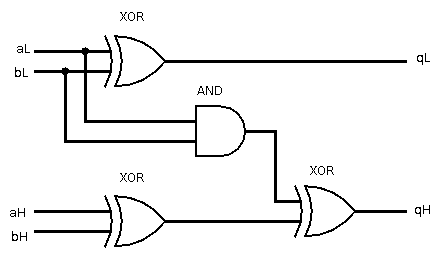
\includegraphics[scale=0.75]{SAT/adder_logisim.png}
\caption{2-bit adder schematics}
\end{figure}

The adder in its simplest form: it has no carry-in and carry-out, and it has 3 XOR gates and one AND gate.
Let's try to figure out, which sets of inputs will force adder to set both two output bits?
By doing quick memory calculation, we can see that there are 4 ways to do so: $0+3=3$, $1+2=3$, $2+1=3$, $3+0=3$.
Here is also truth table, with these rows highlighted:

\newcommand{\HLcell}{\cellcolor{blue!25}}

\begin{center}
\begin{doublespace}
\noindent\(\begin{array}{l|llllll}
  & \text{aH} & \text{aL} & \text{bH} & \text{bL} & \text{qH} & \text{qL} \\
\hline
 \text{3+3 = 6 $\equiv $ 2 (mod 4)} & 1 & 1 & 1 & 1 & 1 & 0 \\
 \text{3+2 = 5 $\equiv $ 1 (mod 4)} & 1 & 1 & 1 & 0 & 0 & 1 \\
 \text{3+1 = 4 $\equiv $ 0 (mod 4)} & 1 & 1 & 0 & 1 & 0 & 0 \\
 \text{\HLcell{}3+0 = 3 $\equiv $ 3 (mod 4)} & \HLcell{}1 & \HLcell{}1 & \HLcell{}0 & \HLcell{}0 & \HLcell{}1 & \HLcell{}1 \\
 \text{2+3 = 5 $\equiv $ 1 (mod 4)} & 1 & 0 & 1 & 1 & 0 & 1 \\
 \text{2+2 = 4 $\equiv $ 0 (mod 4)} & 1 & 0 & 1 & 0 & 0 & 0 \\
 \text{\HLcell{}2+1 = 3 $\equiv $ 3 (mod 4)} & \HLcell{}1 & \HLcell{}0 & \HLcell{}0 & \HLcell{}1 & \HLcell{}1 & \HLcell{}1 \\
 \text{2+0 = 2 $\equiv $ 2 (mod 4)} & 1 & 0 & 0 & 0 & 1 & 0 \\
 \text{1+3 = 4 $\equiv $ 0 (mod 4)} & 0 & 1 & 1 & 1 & 0 & 0 \\
 \text{\HLcell{}1+2 = 3 $\equiv $ 3 (mod 4)} & \HLcell{}0 & \HLcell{}1 & \HLcell{}1 & \HLcell{}0 & \HLcell{}1 & \HLcell{}1 \\
 \text{1+1 = 2 $\equiv $ 2 (mod 4)} & 0 & 1 & 0 & 1 & 1 & 0 \\
 \text{1+0 = 1 $\equiv $ 1 (mod 4)} & 0 & 1 & 0 & 0 & 0 & 1 \\
 \text{\HLcell{}0+3 = 3 $\equiv $ 3 (mod 4)} & \HLcell{}0 & \HLcell{}0 & \HLcell{}1 & \HLcell{}1 & \HLcell{}1 & \HLcell{}1 \\
 \text{0+2 = 2 $\equiv $ 2 (mod 4)} & 0 & 0 & 1 & 0 & 1 & 0 \\
 \text{0+1 = 1 $\equiv $ 1 (mod 4)} & 0 & 0 & 0 & 1 & 0 & 1 \\
 \text{0+0 = 0 $\equiv $ 0 (mod 4)} & 0 & 0 & 0 & 0 & 0 & 0 \\
\end{array}\)
\end{doublespace}
\end{center}

Let's find, what \ac{SAT}-solver can say about it?

First, we should represent our 2-bit adder as CNF expression.

Using Wolfram Mathematica, I'll express 1-bit expressions for both adder outputs:\\
\\
\textbf{\texttt{In[]:=AdderQ0[aL$\_$,bL$\_$]=Xor[aL,bL]}} \\
\textbf{\texttt{Out[]:=aL $\veebar$ bL}} \\
\\
\textbf{\texttt{In[]:=AdderQ1[aL$\_$,aH$\_$,bL$\_$,bH$\_$]=Xor[And[aL,bL],Xor[aH,bH]]}} \\
\textbf{\texttt{Out[]:=aH $\veebar$ bH $\veebar$ (aL \&\& bL)}} \\
\\
We need such expression, where both parts will generate 1's.
Let's use Wolfram Mathematica find all instances of such expression (I glueled both parts with And): \\
\\
\textbf{\texttt{In[]:=Boole[SatisfiabilityInstances[And[AdderQ0[aL,bL],AdderQ1[aL,aH,bL,bH]],\{aL,aH,bL,bH\},4]]}} \\
\textbf{\texttt{Out[]:=\{1,1,0,0\},\{1,0,0,1\},\{0,1,1,0\},\{0,0,1,1\}}} \\
\\
Yes, indeed, Mathematica says, there are 4 inputs which will lead to the result we need.
So, Mathematica can also be used as \ac{SAT} solver.

Nevertheless, let's proceed to CNF form. Using Mathematica again, let's convert our expression to CNF form:\\
\\
\textbf{\texttt{In[]:=cnf=BooleanConvert[And[AdderQ0[aL,bL],AdderQ1[aL,aH,bL,bH]],``CNF'']}} \\
\textbf{\texttt{Out[]:=(!aH $\|$ !bH) \&\& (aH $\|$ bH) \&\& (!aL $\|$ !bL) \&\& (aL $\|$ bL)}} \\
\\
Looks more complex. The reason of such verbosity is that CNF form doesn't allow XOR operations.
% FIXME: TeX form of the expression!

\subsubsection{MiniSat}

For the starters, we can try MiniSat\footnote{\url{http://minisat.se/MiniSat.html}}.
The standard way to encode CNF expression for MiniSat is to enumerate all OR parts at each line.
Also, MiniSat doesn't support variable names, just numbers.
Let's enumerate our variables: 1 will be aH, 2 -- aL, 3 -- bH, 4 -- bL.

Here is what I've got when I converted Mathematica expression to the MiniSat input file:

\begin{lstlisting}
p cnf 4 4
-1 -3 0
1 3 0
-2 -4 0
2 4 0
\end{lstlisting}

Two 4's at the first lines are number of variables and number of clauses respectively.
There are 4 lines then, each for each OR clause.
Minus before variable number meaning that the variable is negated.
Absence of minus -- not negated.
Zero at the end is just terminating zero, meaning end of the clause.

In other words, each line is OR-clause with optional negation, and the task of MiniSat is to find such set of input, which can satisfy all lines
in the input file.

The following file I named as \textit{adder.cnf} and now let's try MiniSat:

\begin{lstlisting}
% minisat -verb=0 adder.cnf results.txt
SATISFIABLE
\end{lstlisting}

The results are in \textit{results.txt} file:

\begin{lstlisting}
SAT
-1 -2 3 4 0
\end{lstlisting}

This means, if the first two variables (aH and aL) will be \textit{false}, and the last two variables (bH and bL) will be set to \textit{true},
the whole CNF expression is satisfiable.
Seems to be true: if bH and bL are the only inputs set to \textit{true}, both resulting bits are also has \textit{true} states.

Now how to get other instances? \ac{SAT}-solvers, like \ac{SMT} solvers, produce only one solution (or \textit{instance}).

MiniSat uses PRNG and its initial seed can be set explicitely. I tried different values, but result is still the same.
Nevertheless, CryptoMiniSat in this case was able to show all possible 4 instances, in chaotic order, though.
So this is not very robust way.

Perhaps, the only known way is to negate solution clause and add it to the input expression.
We've got \TT{-1 -2 3 4}, 
now we can negate all variables in it (just toggle minuses: \TT{1 2 -3 -4} and add it to the end of the input file:

\begin{lstlisting}
p cnf 4 5
-1 -3 0
1 3 0
-2 -4 0
2 4 0
1 2 -3 -4
\end{lstlisting}

Now we've got another result:

\begin{lstlisting}
SAT
1 2 -3 -4 0
\end{lstlisting}

This means, aH and aL must be both \textit{true} and bH and bL must be \textit{false}, to satisfy the input expression.
Let's negate this clause and add it again:

\begin{lstlisting}
p cnf 4 6
-1 -3 0
1 3 0
-2 -4 0
2 4 0
1 2 -3 -4
-1 -2 3 4 0
\end{lstlisting}

The result is

\begin{lstlisting}
SAT
-1 2 3 -4 0
\end{lstlisting}

aH=false, aL=true, bH=true, bL=false. This is also correct, according to our truth table.

Let's add it again:

\begin{lstlisting}
p cnf 4 7
-1 -3 0
1 3 0
-2 -4 0
2 4 0
1 2 -3 -4
-1 -2 3 4 0
1 -2 -3 4 0
\end{lstlisting}

\begin{lstlisting}
SAT
1 -2 -3 4 0
\end{lstlisting}

aH=true, aL=false, bH=false, bL=true. This is also correct.

This is fourth result. There are shouldn't be more. What if to add it?

\begin{lstlisting}
p cnf 4 8
-1 -3 0
1 3 0
-2 -4 0
2 4 0
1 2 -3 -4
-1 -2 3 4 0
1 -2 -3 4 0
-1 2 3 -4 0
\end{lstlisting}

Now MiniSat just says ``UNSATISFIABLE'' without any additional information in the resulting file.

Our example is tiny, but MiniSat can work with huge CNF expressions.

\subsubsection{CryptoMiniSat}

XOR operation is absent in CNF form, but crucial in cryptographical algorithms.
Simplest possible way to represent single XOR operation in CNF form is: $(\neg x \vee \neg y) \wedge (x \vee y)$ -- not that small expression, 
though, many XOR operations in single expression can be optimized better.

One significant difference between MiniSat and CryptoMiniSat is that the latter supports CNF clauses with XOR operations instead of ORs,
because CryptoMiniSat has aim to analyze some of crypto algorithms\footnote{\url{http://www.msoos.org/xor-clauses/}}.
XOR clauses are handled by CryptoMiniSat in a special way without translating to OR clauses.

You need just to prepend a clause with ``x'' in .cnf file and OR clause is then treated as XOR clause by CryptoMiniSat.
As of 2-bit adder, this smallest possible XOR-CNF expression can be used to find all inputs where both output adder bits are set:

$(aH \oplus bH) \wedge (aL \oplus bL)$

This is 2-bit adder \TT{.cnf} file for CryptoMiniSat:

\begin{lstlisting}
p cnf 4 2
x1 3 0
x2 4 0
\end{lstlisting}

Now I run CryptoMiniSat with various random seeds...

\begin{lstlisting}
% cryptominisat4 --verb 0 --random 0 XOR_adder.cnf
s SATISFIABLE
v 1 2 -3 -4 0
% cryptominisat4 --verb 0 --random 1 XOR_adder.cnf
s SATISFIABLE
v -1 -2 3 4 0
% cryptominisat4 --verb 0 --random 2 XOR_adder.cnf
s SATISFIABLE
v 1 -2 -3 4 0
% cryptominisat4 --verb 0 --random 3 XOR_adder.cnf
s SATISFIABLE
v 1 2 -3 -4 0
% cryptominisat4 --verb 0 --random 4 XOR_adder.cnf
s SATISFIABLE
v -1 2 3 -4 0
% cryptominisat4 --verb 0 --random 5 XOR_adder.cnf
s SATISFIABLE
v -1 2 3 -4 0
% cryptominisat4 --verb 0 --random 6 XOR_adder.cnf
s SATISFIABLE
v -1 -2 3 4 0
% cryptominisat4 --verb 0 --random 7 XOR_adder.cnf
s SATISFIABLE
v 1 -2 -3 4 0
% cryptominisat4 --verb 0 --random 8 XOR_adder.cnf
s SATISFIABLE
v 1 2 -3 -4 0
% cryptominisat4 --verb 0 --random 9 XOR_adder.cnf
s SATISFIABLE
v 1 2 -3 -4 0
\end{lstlisting}

Nevertheless, all 4 possible solutions are:

\begin{lstlisting}
v -1 -2 3 4 0
v -1 2 3 -4 0
v 1 -2 -3 4 0
v 1 2 -3 -4 0
\end{lstlisting}

The same as reported by MiniSat.

% subsections:
\subsection{Cracking Minesweeper with SAT solver}
\label{minesweeper_SAT}

See also about cracking it using Z3: \ref{minesweeper_SMT}.

SAT solvers are very different in that sense that they are at low-level, and can take only CNF expressions on input.

\subsubsection{Simple population count function}

First of all, somehow we need to count neighbour bombs.
The counting function is very similar to \textit{population count} function.

We can try to make CNF expression in Wolfram Mathematica.
This will be a function, returning True if any of 2 bits of 8 inputs bits are True and others are False.
First, we make truth table of such function:

\begin{lstlisting}
In[]:= tbl2 = 
 Table[PadLeft[IntegerDigits[i, 2], 8] -> 
   If[Equal[DigitCount[i, 2][[1]], 2], 1, 0], {i, 0, 255}]

Out[]= {{0, 0, 0, 0, 0, 0, 0, 0} -> 0, {0, 0, 0, 0, 0, 0, 0, 1} -> 0, 
{0, 0, 0, 0, 0, 0, 1, 0} -> 0, {0, 0, 0, 0, 0, 0, 1, 1} -> 1, 
{0, 0, 0, 0, 0, 1, 0, 0} -> 0, {0, 0, 0, 0, 0, 1, 0, 1} -> 1, 
{0, 0, 0, 0, 0, 1, 1, 0} -> 1, {0, 0, 0, 0, 0, 1, 1, 1} -> 0, 
{0, 0, 0, 0, 1, 0, 0, 0} -> 0, {0, 0, 0, 0, 1, 0, 0, 1} -> 1, 
{0, 0, 0, 0, 1, 0, 1, 0} -> 1, {0, 0, 0, 0, 1, 0, 1, 1} -> 0, 
...
{1, 1, 1, 1, 1, 0, 1, 0} -> 0, {1, 1, 1, 1, 1, 0, 1, 1} -> 0, 
{1, 1, 1, 1, 1, 1, 0, 0} -> 0, {1, 1, 1, 1, 1, 1, 0, 1} -> 0, 
{1, 1, 1, 1, 1, 1, 1, 0} -> 0, {1, 1, 1, 1, 1, 1, 1, 1} -> 0}
\end{lstlisting}

Now we can make CNF expression using this truth table:

\begin{lstlisting}
In[]:= BooleanConvert[
 BooleanFunction[tbl2, {a, b, c, d, e, f, g, h}], "CNF"]

Out[]= (! a || ! b || ! c) && (! a || ! b || ! d) && (! a || ! 
    b || ! e) && (! a || ! b || ! f) && (! a || ! b || ! g) && (! 
    a || ! b || ! h) && (! a || ! c || ! d) && (! a || ! c || ! 
    e) && (! a || ! c || ! f) && (! a || ! c || ! g) && (! a || ! 
    c || ! h) && (! a || ! d || ! e) && (! a || ! d || ! f) && (! 
    a || ! d || ! g) && (! a || ! d || ! h) && (! a || ! e || ! 
    f) && (! a || ! e || ! g) && (! a || ! e || ! h) && (! a || ! 
    f || ! g) && (! a || ! f || ! h) && (! a || ! g || ! h) && (a || 
   b || c || d || e || f || g) && (a || b || c || d || e || f || 
   h) && (a || b || c || d || e || g || h) && (a || b || c || d || f ||
    g || h) && (a || b || c || e || f || g || h) && (a || b || d || 
   e || f || g || h) && (a || c || d || e || f || g || 
   h) && (! b || ! c || ! d) && (! b || ! c || ! e) && (! b || ! 
    c || ! f) && (! b || ! c || ! g) && (! b || ! c || ! h) && (! 
    b || ! d || ! e) && (! b || ! d || ! f) && (! b || ! d || ! 
    g) && (! b || ! d || ! h) && (! b || ! e || ! f) && (! b || ! 
    e || ! g) && (! b || ! e || ! h) && (! b || ! f || ! g) && (! 
    b || ! f || ! h) && (! b || ! g || ! h) && (b || c || d || e || 
   f || g || 
   h) && (! c || ! d || ! e) && (! c || ! d || ! f) && (! c || ! 
    d || ! g) && (! c || ! d || ! h) && (! c || ! e || ! f) && (! 
    c || ! e || ! g) && (! c || ! e || ! h) && (! c || ! f || ! 
    g) && (! c || ! f || ! h) && (! c || ! g || ! h) && (! d || ! 
    e || ! f) && (! d || ! e || ! g) && (! d || ! e || ! h) && (! 
    d || ! f || ! g) && (! d || ! f || ! h) && (! d || ! g || ! 
    h) && (! e || ! f || ! g) && (! e || ! f || ! h) && (! e || ! 
    g || ! h) && (! f || ! g || ! h)
\end{lstlisting}

The syntax is similar to C/C++.
Let's check it.

I wrote a Python function to convert Mathematica's output into CNF file which can be feeded to SAT solver:

\lstinputlisting{SAT/minesweeper/tst.py}

It replaces a/b/c/... variables to the variable names passed (1/2/3...), reworks syntax, etc.
Here is a result:

\lstinputlisting{SAT/minesweeper/tst1.cnf}

I can run it:

\begin{lstlisting}
% minisat -verb=0 tst1.cnf results.txt
WARNING: for repeatability, setting FPU to use double precision
SATISFIABLE

% cat results.txt
SAT
1 -2 -3 -4 -5 -6 -7 8 0
\end{lstlisting}

The variable name in results lacking minus sign is "True".
Variable name with minus sign is "False".
We see there are just two variables are "True": 1 and 8.
This is indeed correct: MiniSat solver found a condition, for which our function returns "True".
Zero at the end is just a terminal symbol which means nothing.

We can ask MiniSat for another solution, by adding current solution to the input CNF file, but with all variables negated:

\begin{lstlisting}
...
-5 -6 -8 0
-5 -7 -8 0
-6 -7 -8 0
-1 2 3 4 5 6 7 -8 0
\end{lstlisting}

In plain English language, this means "give me ANY solution which can satisfy all clauses, but also not equal to the last clause we've just added".

MiniSat, indeed, found another solution, again, with only 2 variables equal to "True":

\begin{lstlisting}
% minisat -verb=0 tst2.cnf results.txt
WARNING: for repeatability, setting FPU to use double precision
SATISFIABLE

% cat results.txt
SAT
1 2 -3 -4 -5 -6 -7 -8 0
\end{lstlisting}

By the way, <i>population count</i> function for 8 neighbours in CNF form is simplest:

\begin{lstlisting}
a&&b&&c&&d&&e&&f&&g&&h
\end{lstlisting}

Indeed: it's true if all 8 input bits are "True".

The function for 0 neighbours is also simple:

\begin{lstlisting}
!a&&!b&&!c&&!d&&!e&&!f&&!g&&!h
\end{lstlisting}

It means, it will return "True", if all input variables are "False".

By the way, function for POPCNT1 is also simple:

\begin{lstlisting}
(!a||!b)&&(!a||!c)&&(!a||!d)&&(!a||!e)&&(!a||!f)&&(!a||!g)&&(!a||!h)&&(a||b||c||d||e||f||g||h)&&
(!b||!c)&&(!b||!d)&&(!b||!e)&&(!b||!f)&&(!b||!g)&&(!b||!h)&&(!c||!d)&&(!c||!e)&&(!c||!f)&&(!c||!g)&&
(!c||!h)&&(!d||!e)&&(!d||!f)&&(!d||!g)&&(!d||!h)&&(!e||!f)&&(!e||!g)&&(!e||!h)&&(!f||!g)&&(!f||!h)&&(!g||!h)
\end{lstlisting}

It just enumerates all possible pairs of 8 variables (a/b, a/c, a/d, etc) and says: no two bits must be present
simultaneously in each possible pair.
And there is another clause: "(a||b||c||d||e||f||g||h)", which says: at least one bit must be present among 8 variables.

And yes, you can ask Mathematica for finding CNF expressions for any other truth table.

\subsubsection{Minesweeper}

Now we can use Mathematica to get all \textit{population count} functions for 0..8 neighbours.

For 9*9 Minesweeper grid including invisible border, there will be 11*11=121 variables, mapped to Minesweeper grid like this:

\begin{lstlisting}
 1    2   3   4   5   6   7   8   9  10  11
12   13  14  15  16  17  18  19  20  21  22
23   24  25  26  27  28  29  30  31  32  33
34   35  36  37  38  39  40  41  42  43  44

...

100 101 102 103 104 105 106 107 108 109 110
111 112 113 114 115 116 117 118 119 120 121
\end{lstlisting}

Then we write a Python script which stacks all \textit{population count} functions: each function for each known number of neighbours (digit on Minesweeper field).
Each POPCNTx() function takes list of variable numbers and outputs list of clauses to be added to the final CNF file.

As of empty cells, we also add them as clauses, but with minus sign, which means, the variable must be False.
Whenever we try to place bomb, we add its variable as clause without minus sign, this means the variable must be True.

Then we execute external minisat process.
The only thing we need from it is exit code.
If an input CNF is UNSAT, it returns 20:

\lstinputlisting{SAT/minesweeper/minesweeper_SAT.py}

The output CNF file can be large, up to ~2000 clauses, or more, here is an example: \url{https://github.com/dennis714/SAT_SMT_article/blob/master/SAT/minesweeper/sample.cnf}.

Anyway, it works just like my previous Z3Py script:

\begin{lstlisting}
row=1, col=3, unsat!
row=6, col=2, unsat!
row=6, col=3, unsat!
row=7, col=4, unsat!
row=7, col=9, unsat!
row=8, col=9, unsat!
\end{lstlisting}

... but it runs way faster, even considering overhead of executing external program.
Perhaps, Z3Py version could be optimized much better?

The files, including Wolfram Mathematica notebook: \url{https://github.com/dennis714/SAT_SMT_article/tree/master/SAT/minesweeper}.


\subsection{Conway's Game of Life and SAT solver}

\subsubsection{Part I: reversing back state of ``Game of Life''}

How could we reverse back a known state of GoL?
This can be solved by brute-force, but this is extremely slow and inefficient.

Let's try to use SAT solver.

First, we need to define a function which will tell, if the new cell will be created/born, preserved/stay or died.
Quick refresher: cell is born if it has 3 neighbours, it stays alive if it has 2 or 3 neighbours, it dies in any other case.

This is how I can define a function reflecting state of a new cell in the next state:

\begin{lstlisting}
if center==true:
	return popcnt2(neighbours) || popcnt3(neighbours)
if center==false
	return popcnt3(neighbours)
\end{lstlisting}

We can get rid of ``if'' construction:

\begin{lstlisting}
result=(center=true && (popcnt2(neighbours) || popcnt3(neighbours))) || (center=false && popcnt3(neighbours))
\end{lstlisting}

... where ``center'' is state of central cell, ``neighbours'' are 8 neighbouring cells, popcnt2 is a function which
returns True if it has exactly 2 bits on input, popcnt3 is the same, but for 3 bits
(just like these were used in my "Minesweeper" example (\ref{minesweeper_SAT}).

Using Wolfram Mathematica, I first create all helper functions and truth table for the function, which returns "true",
if a cell must be present in the next state, or "false" if not:

\begin{lstlisting}
In[1]:= popcount[n_Integer]:=IntegerDigits[n,2] // Total

In[2]:= popcount2[n_Integer]:=Equal[popcount[n],2]

In[3]:= popcount3[n_Integer]:=Equal[popcount[n],3]

In[4]:= newcell[center_Integer,neighbours_Integer]:=(center==1 && (popcount2[neighbours]|| popcount3[neighbours]))||
(center==0 && popcount3[neighbours])

In[13]:= NewCellIsTrue=Flatten[Table[Join[{center},PadLeft[IntegerDigits[neighbours,2],8]] ->
Boole[newcell[center, neighbours]],{neighbours,0,255},{center,0,1}]]

Out[13]= {{0,0,0,0,0,0,0,0,0}->0,
{1,0,0,0,0,0,0,0,0}->0,
{0,0,0,0,0,0,0,0,1}->0,
{1,0,0,0,0,0,0,0,1}->0,
{0,0,0,0,0,0,0,1,0}->0,
{1,0,0,0,0,0,0,1,0}->0,
{0,0,0,0,0,0,0,1,1}->0,
{1,0,0,0,0,0,0,1,1}->1,

...

\end{lstlisting}

Now we can create a CNF expression out of truth table:

\begin{lstlisting}
In[14]:= BooleanConvert[BooleanFunction[NewCellIsTrue,{center,a,b,c,d,e,f,g,h}],"CNF"]
Out[14]= (!a||!b||!c||!d)&&(!a||!b||!c||!e)&&(!a||!b||!c||!f)&&(!a||!b||!c||!g)&&(!a||!b||!c||!h)&&(!a||!b||!d||!e)&&
(!a||!b||!d||!f)&&(!a||!b||!d||!g)&&(!a||!b||!d||!h)&&(!a||!b||!e||!f)&&(!a||!b||!e||!g)&&(!a||!b||!e||!h)&&
(!a||!b||!f||!g)&&(!a||!b||!f||!h)&&(!a||!b||!g||!h)&&(!a||!c||!d||!e)&&(!a||!c||!d||!f)&&(!a||!c||!d||!g)&&
(!a||!c||!d||!h)&&(!a||!c||!e||!f)&&(!a||!c||!e||!g)&&(!a||!c||!e||!h)&&(!a||!c||!f||!g)&&(!a||!c||!f||!h)&&

...

\end{lstlisting}

Also, we need a second function, "inverted" one, which will return "true" if the cell must be absent in the next state,
or "false" otherwise:

\begin{lstlisting}
In[15]:= NewCellIsFalse=Flatten[Table[Join[{center},PadLeft[IntegerDigits[neighbours,2],8]] ->
Boole[Not[newcell[center, neighbours]]],{neighbours,0,255},{center,0,1}]]
Out[15]= {{0,0,0,0,0,0,0,0,0}->1,
{1,0,0,0,0,0,0,0,0}->1,
{0,0,0,0,0,0,0,0,1}->1,
{1,0,0,0,0,0,0,0,1}->1,
{0,0,0,0,0,0,0,1,0}->1,

...

In[16]:= BooleanConvert[BooleanFunction[NewCellIsFalse,{center,a,b,c,d,e,f,g,h}],"CNF"]
Out[16]= (!a||!b||!c||d||e||f||g||h)&&(!a||!b||c||!d||e||f||g||h)&&(!a||!b||c||d||!e||f||g||h)&&
(!a||!b||c||d||e||!f||g||h)&&(!a||!b||c||d||e||f||!g||h)&&(!a||!b||c||d||e||f||g||!h)&&
(!a||!b||!center||d||e||f||g||h)&&(!a||b||!c||!d||e||f||g||h)&&(!a||b||!c||d||!e||f||g||h)&&
(!a||b||!c||d||e||!f||g||h)&&(!a||b||!c||d||e||f||!g||h)&&(!a||b||!c||d||e||f||g||!h)&&
(!a||b||c||!d||!e||f||g||h)&&(!a||b||c||!d||e||!f||g||h)&&(!a||b||c||!d||e||f||!g||h)&&

...

\end{lstlisting}

Using the very same way as in my "Minesweeper" example, I can convert CNF expression to list of clauses:

\begin{lstlisting}
def mathematica_to_CNF (s, center, a):
    s=s.replace("center", center)
    s=s.replace("a", a[0]).replace("b", a[1]).replace("c", a[2]).replace("d", a[3])
    s=s.replace("e", a[4]).replace("f", a[5]).replace("g", a[6]).replace("h", a[7])
    s=s.replace("!", "-").replace("||", " ").replace("(", "").replace(")", "")
    s=s.split ("&&")
    return s
\end{lstlisting}

And again, as in "Minesweeper", there is an invisible border, to make processing simpler.
SAT variables are also numbered as in previous example:

\begin{lstlisting}
 1    2   3   4   5   6   7   8   9  10  11
12   13  14  15  16  17  18  19  20  21  22
23   24  25  26  27  28  29  30  31  32  33
34   35  36  37  38  39  40  41  42  43  44

...

100 101 102 103 104 105 106 107 108 109 110
111 112 113 114 115 116 117 118 119 120 121
\end{lstlisting}

Also, there is a visible border, always fixed to "False", to make things simpler.

Now the working source code.
Whenever we encounter "*" in final\_state[], we add clauses generated by cell\_is\_true() function,
or cell\_is\_false() if otherwise.
When we get a solution, it is negated and added to the list of clauses, so when minisat is executed next time,
it will skip solution which was already printed.

\begin{lstlisting}
...

def cell_is_false (center, a):
    s="(!a||!b||!c||d||e||f||g||h)&&(!a||!b||c||!d||e||f||g||h)&&(!a||!b||c||d||!e||f||g||h)&&" \
      "(!a||!b||c||d||e||!f||g||h)&&(!a||!b||c||d||e||f||!g||h)&&(!a||!b||c||d||e||f||g||!h)&&" \
      "(!a||!b||!center||d||e||f||g||h)&&(!a||b||!c||!d||e||f||g||h)&&(!a||b||!c||d||!e||f||g||h)&&" \
      "(!a||b||!c||d||e||!f||g||h)&&(!a||b||!c||d||e||f||!g||h)&&(!a||b||!c||d||e||f||g||!h)&&" \
      "(!a||b||c||!d||!e||f||g||h)&&(!a||b||c||!d||e||!f||g||h)&&(!a||b||c||!d||e||f||!g||h)&&" \
      "(!a||b||c||!d||e||f||g||!h)&&(!a||b||c||d||!e||!f||g||h)&&(!a||b||c||d||!e||f||!g||h)&&" \
      "(!a||b||c||d||!e||f||g||!h)&&(!a||b||c||d||e||!f||!g||h)&&(!a||b||c||d||e||!f||g||!h)&&" \
      "(!a||b||c||d||e||f||!g||!h)&&(!a||!c||!center||d||e||f||g||h)&&(!a||c||!center||!d||e||f||g||h)&&" \
      "(!a||c||!center||d||!e||f||g||h)&&(!a||c||!center||d||e||!f||g||h)&&(!a||c||!center||d||e||f||!g||h)&&" \
      "(!a||c||!center||d||e||f||g||!h)&&(a||!b||!c||!d||e||f||g||h)&&(a||!b||!c||d||!e||f||g||h)&&" \
      "(a||!b||!c||d||e||!f||g||h)&&(a||!b||!c||d||e||f||!g||h)&&(a||!b||!c||d||e||f||g||!h)&&" \
      "(a||!b||c||!d||!e||f||g||h)&&(a||!b||c||!d||e||!f||g||h)&&(a||!b||c||!d||e||f||!g||h)&&" \
      "(a||!b||c||!d||e||f||g||!h)&&(a||!b||c||d||!e||!f||g||h)&&(a||!b||c||d||!e||f||!g||h)&&" \
      "(a||!b||c||d||!e||f||g||!h)&&(a||!b||c||d||e||!f||!g||h)&&(a||!b||c||d||e||!f||g||!h)&&" \
      "(a||!b||c||d||e||f||!g||!h)&&(a||b||!c||!d||!e||f||g||h)&&(a||b||!c||!d||e||!f||g||h)&&" \
      "(a||b||!c||!d||e||f||!g||h)&&(a||b||!c||!d||e||f||g||!h)&&(a||b||!c||d||!e||!f||g||h)&&" \
      "(a||b||!c||d||!e||f||!g||h)&&(a||b||!c||d||!e||f||g||!h)&&(a||b||!c||d||e||!f||!g||h)&&" \
      "(a||b||!c||d||e||!f||g||!h)&&(a||b||!c||d||e||f||!g||!h)&&(a||b||c||!d||!e||!f||g||h)&&" \
      "(a||b||c||!d||!e||f||!g||h)&&(a||b||c||!d||!e||f||g||!h)&&(a||b||c||!d||e||!f||!g||h)&&" \
      "(a||b||c||!d||e||!f||g||!h)&&(a||b||c||!d||e||f||!g||!h)&&(a||b||c||d||!e||!f||!g||h)&&" \
      "(a||b||c||d||!e||!f||g||!h)&&(a||b||c||d||!e||f||!g||!h)&&(a||b||c||d||e||!f||!g||!h)&&" \
      "(!b||!c||!center||d||e||f||g||h)&&(!b||c||!center||!d||e||f||g||h)&&(!b||c||!center||d||!e||f||g||h)&&" \
      "(!b||c||!center||d||e||!f||g||h)&&(!b||c||!center||d||e||f||!g||h)&&(!b||c||!center||d||e||f||g||!h)&&" \
      "(b||!c||!center||!d||e||f||g||h)&&(b||!c||!center||d||!e||f||g||h)&&(b||!c||!center||d||e||!f||g||h)&&" \
      "(b||!c||!center||d||e||f||!g||h)&&(b||!c||!center||d||e||f||g||!h)&&(b||c||!center||!d||!e||f||g||h)&&" \
      "(b||c||!center||!d||e||!f||g||h)&&(b||c||!center||!d||e||f||!g||h)&&(b||c||!center||!d||e||f||g||!h)&&" \
      "(b||c||!center||d||!e||!f||g||h)&&(b||c||!center||d||!e||f||!g||h)&&(b||c||!center||d||!e||f||g||!h)&&" \
      "(b||c||!center||d||e||!f||!g||h)&&(b||c||!center||d||e||!f||g||!h)&&(b||c||!center||d||e||f||!g||!h)"

    return mathematica_to_CNF(s, center, a)

def cell_is_true (center, a):
    s="(!a||!b||!c||!d)&&(!a||!b||!c||!e)&&(!a||!b||!c||!f)&&(!a||!b||!c||!g)&&(!a||!b||!c||!h)&&" \
      "(!a||!b||!d||!e)&&(!a||!b||!d||!f)&&(!a||!b||!d||!g)&&(!a||!b||!d||!h)&&(!a||!b||!e||!f)&&" \
      "(!a||!b||!e||!g)&&(!a||!b||!e||!h)&&(!a||!b||!f||!g)&&(!a||!b||!f||!h)&&(!a||!b||!g||!h)&&" \
      "(!a||!c||!d||!e)&&(!a||!c||!d||!f)&&(!a||!c||!d||!g)&&(!a||!c||!d||!h)&&(!a||!c||!e||!f)&&" \
      "(!a||!c||!e||!g)&&(!a||!c||!e||!h)&&(!a||!c||!f||!g)&&(!a||!c||!f||!h)&&(!a||!c||!g||!h)&&" \
      "(!a||!d||!e||!f)&&(!a||!d||!e||!g)&&(!a||!d||!e||!h)&&(!a||!d||!f||!g)&&(!a||!d||!f||!h)&&" \
      "(!a||!d||!g||!h)&&(!a||!e||!f||!g)&&(!a||!e||!f||!h)&&(!a||!e||!g||!h)&&(!a||!f||!g||!h)&&" \
      "(a||b||c||center||d||e||f)&&(a||b||c||center||d||e||g)&&(a||b||c||center||d||e||h)&&" \
      "(a||b||c||center||d||f||g)&&(a||b||c||center||d||f||h)&&(a||b||c||center||d||g||h)&&" \
      "(a||b||c||center||e||f||g)&&(a||b||c||center||e||f||h)&&(a||b||c||center||e||g||h)&&" \
      "(a||b||c||center||f||g||h)&&(a||b||c||d||e||f||g)&&(a||b||c||d||e||f||h)&&(a||b||c||d||e||g||h)&&" \
      "(a||b||c||d||f||g||h)&&(a||b||c||e||f||g||h)&&(a||b||center||d||e||f||g)&&(a||b||center||d||e||f||h)&&" \
      "(a||b||center||d||e||g||h)&&(a||b||center||d||f||g||h)&&(a||b||center||e||f||g||h)&&(a||b||d||e||f||g||h)&&" \
      "(a||c||center||d||e||f||g)&&(a||c||center||d||e||f||h)&&(a||c||center||d||e||g||h)&&" \
      "(a||c||center||d||f||g||h)&&(a||c||center||e||f||g||h)&&(a||c||d||e||f||g||h)&&(a||center||d||e||f||g||h)&&" \
      "(!b||!c||!d||!e)&&(!b||!c||!d||!f)&&(!b||!c||!d||!g)&&(!b||!c||!d||!h)&&(!b||!c||!e||!f)&&" \
      "(!b||!c||!e||!g)&&(!b||!c||!e||!h)&&(!b||!c||!f||!g)&&(!b||!c||!f||!h)&&(!b||!c||!g||!h)&&" \
      "(!b||!d||!e||!f)&&(!b||!d||!e||!g)&&(!b||!d||!e||!h)&&(!b||!d||!f||!g)&&(!b||!d||!f||!h)&&" \
      "(!b||!d||!g||!h)&&(!b||!e||!f||!g)&&(!b||!e||!f||!h)&&(!b||!e||!g||!h)&&(!b||!f||!g||!h)&&" \
      "(b||c||center||d||e||f||g)&&(b||c||center||d||e||f||h)&&(b||c||center||d||e||g||h)&&" \
      "(b||c||center||d||f||g||h)&&(b||c||center||e||f||g||h)&&(b||c||d||e||f||g||h)&&(b||center||d||e||f||g||h)&&" \
      "(!c||!d||!e||!f)&&(!c||!d||!e||!g)&&(!c||!d||!e||!h)&&(!c||!d||!f||!g)&&(!c||!d||!f||!h)&&" \
      "(!c||!d||!g||!h)&&(!c||!e||!f||!g)&&(!c||!e||!f||!h)&&(!c||!e||!g||!h)&&(!c||!f||!g||!h)&&" \
      "(c||center||d||e||f||g||h)&&(!d||!e||!f||!g)&&(!d||!e||!f||!h)&&(!d||!e||!g||!h)&&(!d||!f||!g||!h)&&" \
      "(!e||!f||!g||!h)"

    return mathematica_to_CNF(s, center, a)

...
\end{lstlisting}

( \url{https://github.com/dennis714/SAT_SMT_article/blob/master/SAT/GoL/GoL_SAT_utils.py} )

\lstinputlisting{SAT/GoL/reverse1.py}

( \url{https://github.com/dennis714/SAT_SMT_article/blob/master/SAT/GoL/reverse1.py} )

Here is a result:

\begin{lstlisting}
HEIGHT= 3 WIDTH= 3
2525 clauses
.*.
*.*
.*.
1.rle written

2526 clauses
.**
*..
*.*
2.rle written

2527 clauses
**.
..*
*.*
3.rle written

2528 clauses
*.*
*..
.**
4.rle written

2529 clauses
*.*
..*
**.
5.rle written

2530 clauses
*.*
.*.
*.*
6.rle written

2531 clauses
unsat!
\end{lstlisting}

The first result is the same as input state.
Indeed: this is "still life", i.e., state which will never change, and it is correct solution.
The last solution is also valid.

Now the problem: 2nd, 3rd, 4th and 5th solutions are equivalent to each other, they just mirrored or rotated.
In fact, this is \href{https://en.wikipedia.org/wiki/Reflection_symmetry}{reflectional} (like in mirror) and 
\href{https://en.wikipedia.org/wiki/Rotational_symmetry}{rotational} symmetries.
We can solve this easily: we will take each solution, reflect and rotate it and add them negated to the list of clauses,
so minisat will skip them during its work:

\begin{lstlisting}

...

while True:
    solution=try_again(clauses)
    clauses.append(negate_clause(grid_to_clause(solution, H, W)))
    clauses.append(negate_clause(grid_to_clause(reflect_vertically(solution), H, W)))
    clauses.append(negate_clause(grid_to_clause(reflect_horizontally(solution), H, W)))
    # is this square?
    if W==H:
        clauses.append(negate_clause(grid_to_clause(rotate_square_array(solution,1), H, W)))
        clauses.append(negate_clause(grid_to_clause(rotate_square_array(solution,2), H, W)))
        clauses.append(negate_clause(grid_to_clause(rotate_square_array(solution,3), H, W)))
    print ""

...

\end{lstlisting}

( \url{https://github.com/dennis714/SAT_SMT_article/blob/master/SAT/GoL/reverse2.py} )

Functions reflect\_vertically(), reflect\_horizontally and rotate\_squarearray() are simple array manipulation routines.

Now we get just 3 solutions:

\begin{lstlisting}
HEIGHT= 3 WIDTH= 3
2525 clauses
.*.
*.*
.*.
1.rle written

2531 clauses
.**
*..
*.*
2.rle written

2537 clauses
*.*
.*.
*.*
3.rle written

2543 clauses
unsat!
\end{lstlisting}

This one has only one single ancestor:

\begin{lstlisting}
final_state=[
" * ",
" * ",
" * "]
_PRE_END

_PRE_BEGIN
HEIGHT= 3 WIDTH= 3
2503 clauses
...
***
...
1.rle written

2509 clauses
unsat!
\end{lstlisting}

This is oscillator, of course.

How many states can lead to such picture?

\begin{lstlisting}
final_state=[
"  *  ",
"     ",
" **  ",
"  *  ",
"  *  ",
" *** "]
\end{lstlisting}

28, these are few:

\begin{lstlisting}
HEIGHT= 6 WIDTH= 5
5217 clauses
.*.*.
..*..
.**.*
..*..
..*.*
.**..
1.rle written

5220 clauses
.*.*.
..*..
.**.*
..*..
*.*.*
.**..
2.rle written

5223 clauses
..*.*
..**.
.**..
....*
*.*.*
.**..
3.rle written

5226 clauses
..*.*
..**.
.**..
*...*
..*.*
.**..
4.rle written

...

\end{lstlisting}

Now the biggest, "space invader":

\begin{lstlisting}
final_state=[
"             ",
"   *     *   ",
"    *   *    ",
"   *******   ",
"  ** *** **  ",
" *********** ",
" * ******* * ",
" * *     * * ",
"    ** **    ",
"             "]
\end{lstlisting}

\begin{lstlisting}
HEIGHT= 10 WIDTH= 13
16469 clauses
..*.*.**.....
.....*****...
....**..*....
......*...*..
..**...*.*...
.*..*.*.**..*
*....*....*.*
..*.*..*.....
..*.....*.*..
....**..*.*..
1.rle written

16472 clauses
*.*.*.**.....
.....*****...
....**..*....
......*...*..
..**...*.*...
.*..*.*.**..*
*....*....*.*
..*.*..*.....
..*.....*.*..
....**..*.*..
2.rle written

16475 clauses
..*.*.**.....
*....*****...
....**..*....
......*...*..
..**...*.*...
.*..*.*.**..*
*....*....*.*
..*.*..*.....
..*.....*.*..
....**..*.*..
3.rle written

...

\end{lstlisting}

I don't know how many possible input states can lead to "space invader", perhaps, too many.
Had to stop it.
And it slows down during execution, because number of clauses is increasing (because of negating solutions addition).

All solutions are also exported to RLE files, which can be opened by Golly ( \url{http://golly.sourceforge.net/} ) software.

\subsubsection{Part II: finding "still lives"}

"Still life" in terms of GoL is a state which doesn't change at all.

First, using previous definitions, we will define a truth table of function, which will return true,
if the center cell of the next state is the same as it has been in the previous state, i.e., hasn't been changed:

\begin{lstlisting}
In[17]:= stillife=Flatten[Table[Join[{center},PadLeft[IntegerDigits[neighbours,2],8]]->
Boole[Boole[newcell[center,neighbours]]==center],{neighbours,0,255},{center,0,1}]]
Out[17]= {{0,0,0,0,0,0,0,0,0}->1,
{1,0,0,0,0,0,0,0,0}->0,
{0,0,0,0,0,0,0,0,1}->1,
{1,0,0,0,0,0,0,0,1}->0,

...

In[18]:= BooleanConvert[BooleanFunction[stillife,{center,a,b,c,d,e,f,g,h}],"CNF"]
Out[18]= (!a||!b||!c||!center||!d)&&(!a||!b||!c||!center||!e)&&(!a||!b||!c||!center||!f)&&
(!a||!b||!c||!center||!g)&&(!a||!b||!c||!center||!h)&&(!a||!b||!c||center||d||e||f||g||h)&&
(!a||!b||c||center||!d||e||f||g||h)&&(!a||!b||c||center||d||!e||f||g||h)&&(!a||!b||c||center||d||e||!f||g||h)&&
(!a||!b||c||center||d||e||f||!g||h)&&(!a||!b||c||center||d||e||f||g||!h)&&(!a||!b||!center||!d||!e)&&

...

\end{lstlisting}

\lstinputlisting{SAT/GoL/stillife1.py}

What we've got for 2*2?

\begin{lstlisting}
1881 clauses
..
..
1.rle written

1887 clauses
**
**
2.rle written

1893 clauses
unsat!
\end{lstlisting}

Both solutions are correct: empty square will progress into empty square (no cells are born).
2*2 box is also known still life.

What about 3*3 square?

\begin{lstlisting}
2887 clauses
...
...
...
1.rle written

2893 clauses
.**
.**
...
2.rle written

2899 clauses
.**
*.*
**.
3.rle written

2905 clauses
.*.
*.*
**.
4.rle written

2911 clauses
.*.
*.*
.*.
5.rle written

2917 clauses
unsat!
\end{lstlisting}

Here is a problem: we see familiar 2*2 box, but shifted.
This is indeed correct solution, but we don't interested in it, because it has been already seen.

What we can do is add another condition. We can force minisat to find solutions with no empty rows and columns.
This is easy.
These are SAT variables for 5*5 square:

\begin{lstlisting}
1   2  3  4  5
6   7  8  9 10
11 12 13 14 15
16 17 18 19 20
21 22 23 24 25
\end{lstlisting}

Each clause is "OR" clause, so all we have to do is to add 5 clauses:

\begin{lstlisting}
1 OR 2 OR 3 OR 4 OR 5
6 OR 7 OR 8 OR 9 OR 10

...

\end{lstlisting}

That means that each row must have at least one "True" variable somewhere.
We can also do this for each column as well.

\begin{lstlisting}

...

    # each row must contain at least one cell!
    for r in range(H):
        clauses.append(" ".join([coords_to_var(r, c, H, W) for c in range(W)]))

    # each column must contain at least one cell!
    for c in range(W):
        clauses.append(" ".join([coords_to_var(r, c, H, W) for r in range(H)]))

...

\end{lstlisting}

( \url{https://github.com/dennis714/SAT_SMT_article/blob/master/SAT/GoL/stillife2.py} )

Now we can see that 3*3 square has 3 possible still lives:

\begin{lstlisting}
2893 clauses
.*.
*.*
**.
1.rle written

2899 clauses
.*.
*.*
.*.
2.rle written

2905 clauses
.**
*.*
**.
3.rle written

2911 clauses
unsat!
\end{lstlisting}

4*4 has 7:

\begin{lstlisting}
4169 clauses
..**
...*
***.
*...
1.rle written

4175 clauses
..**
..*.
*.*.
**..
2.rle written

4181 clauses
..**
.*.*
*.*.
**..
3.rle written

4187 clauses
..*.
.*.*
*.*.
**..
4.rle written

4193 clauses
.**.
*..*
*.*.
.*..
5.rle written

4199 clauses
..*.
.*.*
*.*.
.*..
6.rle written

4205 clauses
.**.
*..*
*..*
.**.
7.rle written

4211 clauses
unsat!
\end{lstlisting}

When I try large squares, like 20*20, funny things happen.
First of all, minisat finds solutions not very pleasing aesthetically, but still correct, like:

\begin{lstlisting}
61033 clauses
....**.**.**.**.**.*
**..*.**.**.**.**.**
*...................
.*..................
**..................
*...................
.*..................
**..................
*...................
.*..................
**..................
*...................
.*..................
**..................
*...................
.*..................
..*.................
...*................
***.................
*...................
1.rle written

...

\end{lstlisting}

Indeed: all rows and columns has at least one "True" variable.

Then minisat begins to add smaller "still lives" into the whole picture:

\begin{lstlisting}
61285 clauses
.**....**...**...**.
.**...*..*.*.*...*..
.......**...*......*
..................**
...**............*..
...*.*...........*..
....*.*........**...
**...*.*...**..*....
*.*...*....*....*...
.*..........****.*..
................*...
..*...**..******....
.*.*..*..*..........
*..*...*.*..****....
***.***..*.*....*...
....*..***.**..**...
**.*..*.............
.*.**.**..........**
*..*..*..*......*..*
**..**..**......**..
43.rle written
\end{lstlisting}

In other words, result is a square consisting of smaller "still lives".
It then altering these parts slightly, shifting back and forth.
Is it cheating?
Anyway, it does it in a strict accordance to rules we defined.

But we want "denser" picture. We can add a rule: in all 5-cell chunks there must be at least one "True" cell.
To achieve this, we just split the whole square by 5-cell chunks and add clause for each:

\begin{lstlisting}

...

    # make result denser:
    lst=[]
    for r in range(H):
        for c in range(W):
            lst.append(coords_to_var(r, c, H, W))
    # divide them all by chunks and add to clauses:
    CHUNK_LEN=5
    for c in list_partition(lst,len(lst)/CHUNK_LEN):
        tmp=" ".join(c)
        clauses.append(tmp)

...

\end{lstlisting}

( \url{https://github.com/dennis714/SAT_SMT_article/blob/master/SAT/GoL/stillife.py} )

This is indeed denser:

\begin{lstlisting}
61113 clauses
..**.**......*.*.*..
...*.*.....***.**.*.
...*..*...*.......*.
....*.*..*.*......**
...**.*.*..*...**.*.
..*...*.***.....*.*.
...*.*.*......*..*..
****.*..*....*.**...
*....**.*....*.*....
...**..*...**..*....
..*..*....*....*.**.
.*.*.**....****.*..*
..*.*....*.*..*..**.
....*.****..*..*.*..
....**....*.*.**..*.
*.**...****.*..*.**.
**...**.....**.*....
...**..*..**..*.**.*
***.*.*..*.*..*.*.**
*....*....*....*....
1.rle written

61119 clauses
..**.**......*.*.*..
...*.*.....***.**.*.
...*..*...*.......*.
....*.*..*.*......**
...**.*.*..*...**.*.
..*...*.***.....*.*.
...*.*.*......*..*..
****.*..*....*.**...
*....**.*....*.*....
...**..*...**..*....
..*..*....*....*.**.
.*.*.**....****.*..*
..*.*....*.*..*..**.
....*.****..*..*.*..
....**....*.*.**..*.
*.**...****.*..*.**.
**...**.....**.*....
...**..*.***..*.**.*
***.*..*.*..*.*.*.**
*.......*..**.**....
2.rle written

...

\end{lstlisting}

Let's try more dense, one mandatory "true" cell per each 4-cell chunk:

\begin{lstlisting}
61133 clauses
.**.**...*....**..**
*.*.*...*.*..*..*..*
*....*...*.*..*.**..
.***.*.....*.**.*...
..*.*.....**...*..*.
*......**..*...*.**.
**.....*...*.**.*...
...**...*...**..*...
**.*..*.*......*...*
.*...**.**..***.****
.*....*.*..*..*.*...
**.***...*.**...*.**
.*.*..****.....*..*.
*....*.....**..**.*.
*.***.*..**.*.....**
.*...*..*......**...
...*.*.**......*.***
..**.*.....**......*
*..*.*.**..*.*..***.
**....*.*...*...*...
1.rle written

61139 clauses
.**.**...*....**..**
*.*.*...*.*..*..*..*
*....*...*.*..*.**..
.***.*.....*.**.*...
..*.*.....**...*..*.
*......**..*...*.**.
**.....*...*.**.*...
...**...*...**..*...
**.*..*.*......*...*
.*...**.**..***.****
.*....*.*..*..*.*...
**.***...*.**...*.**
.*.*..****.....*..*.
*....*.....**..**.*.
*.***.*..**.*.....**
.*...*..*......**..*
...*.*.**......*.**.
..**.*.....**....*..
*..*.*.**..*.*...*.*
**....*.*...*.....**
2.rle written

...

\end{lstlisting}

... and even more: one cell per each 3-cell chunk:

\begin{lstlisting}
61166 clauses
**.*..**...**.**....
*.**..*.*...*.*.*.**
....**..*...*...*.*.
.**..*.*.**.*.*.*.*.
..**.*.*...*.**.*.**
*...*.*.**.*....*.*.
**.*..*...*.*.***..*
.*.*.*.***..**...**.
.*.*.*.*..**...*.*..
**.**.*..*...**.*..*
..*...*.**.**.*.*.**
..*.**.*..*.*.*.*...
**.*.*...*..*.*.*...
.*.*...*.**..*..***.
.*..****.*....**...*
..*.*...*..*...*..*.
.**...*.*.**...*.*..
..*..**.*.*...**.**.
..*.*..*..*..*..*..*
.**.**....**..**..**
1.rle written

61172 clauses
**.*..**...**.**....
*.**..*.*...*.*.*.**
....**..*...*...*.*.
.**..*.*.**.*.*.*.*.
..**.*.*...*.**.*.**
*...*.*.**.*....*.*.
**.*..*...*.*.***..*
.*.*.*.***..**...**.
.*.*.*.*..**...*.*..
**.**.*..*...**.*..*
..*...*.**.**.*.*.**
..*.**.*..*.*.*.*...
**.*.*...*..*.*.*...
.*.*...*.**..*..***.
.*..****.*....**...*
..*.*...*..*...*..*.
.**..**.*.**...*.*..
*..*.*..*.*...**.**.
*..*.*.*..*..*..*..*
.**...*...**..**..**
2.rle written

...

\end{lstlisting}

This is most dense. Unfortunaly, it's impossible to construct "still life" with one mandatory "true" cell per each 2-cell chunk.

\subsubsection{The source code}

Source code and Wolfram Mathematica notebook: \url{https://github.com/dennis714/SAT_SMT_article/tree/master/SAT/GoL}.




\section{SMT-solvers}

\subsection{School-level system of equations}

I've got this school-level system of equations copypasted from Wikipedia\footnote{\url{https://en.wikipedia.org/wiki/System_of_linear_equations}}:

\begin{alignat*}{7}
3x &&\; + \;&& 2y             &&\; - \;&& z  &&\; = \;&& 1 & \\
2x &&\; - \;&& 2y             &&\; + \;&& 4z &&\; = \;&& -2 & \\
-x &&\; + \;&& \tfrac{1}{2} y &&\; - \;&& z  &&\; = \;&& 0 &
\end{alignat*}

Will it be possible to solve it using Z3? Here it is:

\begin{lstlisting}
#!/usr/bin/python
from z3 import *

x = Real('x')
y = Real('y')
z = Real('z')
s = Solver()
s.add(3*x + 2*y - z == 1)
s.add(2*x - 2*y + 4*z == -2)
s.add(-x + 0.5*y - z == 0)
print s.check()
print s.model()
\end{lstlisting}

We see this after run:

\begin{lstlisting}
sat
[z = -2, y = -2, x = 1]
\end{lstlisting}

If we change equation in some way so it will have no solution, s.check() will return ``unsat''.

I've used ``Real'' \textit{sort} (some kind of data type in SMT-solvers) because the last expression has $\frac{1}{2}$, which is, of course, a real number.
For the integer system of equations, ``Int'' \textit{sort} would work fine.

Python (and other high-level PLs like C\#) interface is highly popular, because it's practical, but in fact, 
there is a standard language for SMT-solvers named SMT-LIB\cite{SMTLIB}.
Our example rewritten to it looks like this:

\begin{lstlisting}
(declare-const x Real)
(declare-const y Real)
(declare-const z Real)
(assert (=(-(+(* 3 x) (* 2 y)) z) 1))
(assert (=(+(-(* 2 x) (* 2 y)) (* 4 z)) -2))
(assert (=(-(+ (- 0 x) (* 0.5 y)) z) 0))
(check-sat)
(get-model)
\end{lstlisting}

This language is very close to LISP, but hard to read for untrained eyes.

Now we run it:

% FIXME:
\begin{lstlisting}
\$ z3 -smt2 example.smt
sat
(model
  (define-fun z () Real
    (- 2.0))
  (define-fun y () Real
    (- 2.0))
  (define-fun x () Real
    1.0)
)
\end{lstlisting}

So when you look back to my Python code, you may feel that these 3 expressions could be executed.
This is not true: Z3Py API offers overloaded operators, so expressions are constructed and passed into the guts of Z3 without any execution
\footnote{\url{https://github.com/Z3Prover/z3/blob/6e852762baf568af2aad1e35019fdf41189e4e12/src/api/python/z3.py}}.
I would call it ``embedded \ac{DSL}''.

% FIXME \tt, etc
Same thing for Z3 C++ API, you may find there ``operator+'' declarations and many more
\footnote{\url{https://github.com/Z3Prover/z3/blob/6e852762baf568af2aad1e35019fdf41189e4e12/src/api/c\%2B\%2B/z3\%2B\%2B.h}}.

Z3 APIs for Java, ML and .NET are also exist\footnote{\url{https://github.com/Z3Prover/z3/tree/6e852762baf568af2aad1e35019fdf41189e4e12/src/api}}.\\
\\
Z3Py tutorial: \url{https://github.com/ericpony/z3py-tutorial}.

Z3 tutorial which uses SMT-LIB language: \url{http://rise4fun.com/Z3/tutorial/guide}.

\subsection{Another school-level system of equations}

I've found this somewhere at Facebook:

\begin{figure}[H]
\centering
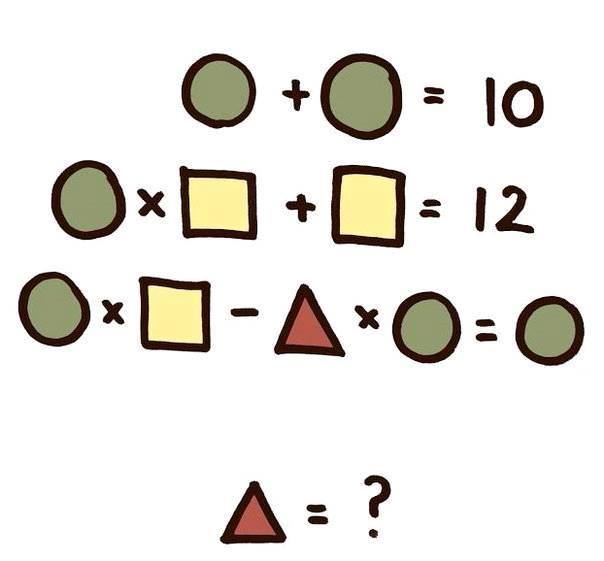
\includegraphics[scale=0.3]{SMT/equation.jpg}
\caption{System of equations}
\end{figure}

It's that easy to solve it in Z3 SMT-solver:

\begin{lstlisting}
#!/usr/bin/python
from z3 import *

circle, square, triangle = Ints('circle square triangle')
s = Solver()
s.add(circle+circle==10)
s.add(circle*square+square==12)
s.add(circle*square-triangle*circle==circle)
print s.check()
print s.model()
\end{lstlisting}

\begin{lstlisting}
sat
[triangle = 1, square = 2, circle = 5]
\end{lstlisting}

\subsection{Connection between SAT and SMT solvers}

Early SMT-solvers were frontends to SAT solvers, i.e., they translating input SMT expressions into \ac{CNF} and feed SAT-solver with it.
Conversion process is sometimes called ``bit blasting''.
Some SMT-solvers still works in that way: STP uses MiniSAT or CryptoMiniSAT as backend SAT-solver.
Some other SMT-solvers are more advanced (like Z3), so they use something even more complex.

% subsections
\subsection{Zebra puzzle (AKA Einstein puzzle)} % FIXME \ac

Zebra puzzle is a popular puzzle, defined as follows:

% FIXME remove paragraph at first line
\begin{framed}
\begin{quotation}
1.There are five houses.\\
2.The Englishman lives in the red house.\\
3.The Spaniard owns the dog.\\
4.Coffee is drunk in the green house.\\
5.The Ukrainian drinks tea.\\
6.The green house is immediately to the right of the ivory house.\\
7.The Old Gold smoker owns snails.\\
8.Kools are smoked in the yellow house.\\
9.Milk is drunk in the middle house.\\
10.The Norwegian lives in the first house.\\
11.The man who smokes Chesterfields lives in the house next to the man with the fox.\\
12.Kools are smoked in the house next to the house where the horse is kept.\\
13.The Lucky Strike smoker drinks orange juice.\\
14.The Japanese smokes Parliaments.\\
15.The Norwegian lives next to the blue house.\\
\\
Now, who drinks water? Who owns the zebra?\\
\\
In the interest of clarity, it must be added that each of the five houses is painted a different color, and their inhabitants are of different national extractions, own different pets, drink different beverages and smoke different brands of American cigarets [sic]. One other thing: in statement 6, right means your right.
\end{quotation}
\end{framed}
( \url{https://en.wikipedia.org/wiki/Zebra_Puzzle} ) \\
\\
It's a very good example of constraint satisfaction problem (CSP). % FIXME \ac

We would encode each entity as integer variable, representing number of house.

Then, to define that Englishman lives in red house, we will define this constraint: \texttt{Englishman == Red}, meaning that number of a house where Englishmen resides and where tea is drunk is the same.

To define that Norwegian lives next to the blue house, we don't realy know, if it is at left side of blue house or at right side, but we know that house numbers are different by just 1.
So we will define this constraint: \texttt{Norwegian==Blue-1 OR Norwegian==Blue+1}.

We will also need to limit all house numbers, so they will be in range of 1..5.

We will also use \texttt{Distinct} to show that all various entities of the same type are all has different house numbers.

\lstinputlisting{SMT/zebra.py}

When we run it, we got correct result:

\begin{lstlisting}
sat
[Snails = 3,
 Blue = 2,
 Ivory = 4,
 OrangeJuice = 4,
 Parliament = 5,
 Yellow = 1,
 Fox = 1,
 Zebra = 5,
 Horse = 2,
 Dog = 4,
 Tea = 2,
 Water = 1,
 Chesterfield = 2,
 Red = 3,
 Japanese = 5,
 LuckyStrike = 4,
 Norwegian = 1,
 Milk = 3,
 Kools = 1,
 OldGold = 3,
 Ukrainian = 2,
 Coffee = 5,
 Green = 5,
 Spaniard = 4,
 Englishman = 3]
 \end{lstlisting}


\subsection{Sudoku puzzle}
\label{sudoku_SMT}

Sudoku puzzle is a 9*9 grid with some cells filled, some are left to be found:

% copypasted from http://www.texample.net/tikz/examples/sudoku/
\newcounter{row}
\newcounter{col}

\newcommand\setrow[9]{
  \setcounter{col}{1}
  \foreach \n in {#1, #2, #3, #4, #5, #6, #7, #8, #9} {
    \edef\x{\value{col} - 0.5}
    \edef\y{9.5 - \value{row}}
    \node[anchor=center] at (\x, \y) {\n};
    \stepcounter{col}
  }
  \stepcounter{row}
}

\begin{center}
\begin{tikzpicture}[scale=.7]
  \begin{scope}
    \draw (0, 0) grid (9, 9);
    \draw[very thick, scale=3] (0, 0) grid (3, 3);

    \setcounter{row}{1}
    \setrow { }{ }{5}  {3}{ }{ }  { }{ }{ }
    \setrow {8}{ }{ }  { }{ }{ }  { }{2}{ }
    \setrow { }{7}{ }  { }{1}{ }  {5}{ }{ }

    \setrow {4}{ }{ }  { }{ }{5}  {3}{ }{ }
    \setrow { }{1}{ }  { }{7}{ }  { }{ }{6}
    \setrow { }{ }{3}  {2}{ }{ }  { }{8}{ }

    \setrow { }{6}{ }  {5}{ }{ }  { }{ }{9}
    \setrow { }{ }{4}  { }{ }{ }  { }{3}{ }
    \setrow { }{ }{ }  { }{ }{9}  {7}{ }{ }

    \node[anchor=center] at (4.5, -0.5) {Unsolved Sudoku};
  \end{scope}
\end{tikzpicture}
\end{center}

Numbers of each row must be unique, i.e., must contain all 9 numbers in range of 1..9 without repetition.
Same story for each column and also for each 3*3 square.

This puzzle is good candidate to try \ac{SMT} solver on, because it's essentially an unsolved system of equations.

\subsubsection{The first idea}

The only thing we must solve is that how to determine in one expression, if the input 9 variables has all 9 unique numbers?
They are not ordered or sorted, after all.

From the school-level mathematics, we can devise this idea:

\begin{equation}
\underbrace{10^{i_1} + 10^{i_2} + \cdots + 10^{i_9}}_9 = 1111111110
\end{equation}

Take each input variable, calculate $10^i$ and sum them all.
If all input values are unique, each will be settled at its own place.
Even more than that: there will be no holes, i.e., no skipped values.
So, in case of Sudoku, 1111111110 number will be final result, indicating that all 9 input variables are unique, in range of 1..9.

Exponentiation is heavy operation, can we use binary operations? Yes, just replace 10 with 2:

\begin{equation}
\underbrace{2^{i_1} + 2^{i_2} + \cdots + 2^{i_9}}_9 = 1111111110_2
\end{equation}

The effect is just the same, but the final value is in base 2 instead of 10.

Now a working example:

\lstinputlisting{SMT/sudoku_plus.py}
( \url{https://github.com/dennis714/SAT_SMT_article/blob/master/SMT/sudoku_plus.py} )

\begin{lstlisting}
% time python sudoku_plus.py
1 4 5 3 2 7 6 9 8
8 3 9 6 5 4 1 2 7
6 7 2 9 1 8 5 4 3
4 9 6 1 8 5 3 7 2
2 1 8 4 7 3 9 5 6
7 5 3 2 9 6 4 8 1
3 6 7 5 4 2 8 1 9
9 8 4 7 6 1 2 3 5
5 2 1 8 3 9 7 6 4

real    0m11.717s
user    0m10.896s
sys     0m0.068s
\end{lstlisting}

Even more, we can replace summing operation to logical OR:

\begin{equation}
\underbrace{2^{i_1} \vee 2^{i_2} \vee \cdots \vee 2^{i_9}}_9 = 1111111110_2
\end{equation}

% FIXME: только часть исходника
\lstinputlisting{SMT/sudoku_or.py}
( \url{https://github.com/dennis714/SAT_SMT_article/blob/master/SMT/sudoku_or.py} )

Now it works much faster. Z3 handles OR operation over bit vectors better than addition?

\begin{lstlisting}
% time python sudoku_or.py
1 4 5 3 2 7 6 9 8
8 3 9 6 5 4 1 2 7
6 7 2 9 1 8 5 4 3
4 9 6 1 8 5 3 7 2
2 1 8 4 7 3 9 5 6
7 5 3 2 9 6 4 8 1
3 6 7 5 4 2 8 1 9
9 8 4 7 6 1 2 3 5
5 2 1 8 3 9 7 6 4

real    0m1.429s
user    0m1.393s
sys     0m0.036s
\end{lstlisting}

The puzzle I used as example is dubbed as one of the hardest known
\footnote{\url{http://www.mirror.co.uk/news/weird-news/worlds-hardest-sudoku-can-you-242294}} (well, for humans).
It took \~1.4 seconds on my Intel Core i3-3110M 2.4GHz notebook to solve it.

\subsubsection{The second idea}

My first approach is far from effective, I did what first came to my mind and worked.
Another approach is to use \TT{distinct} command from SMTLIB, which tells Z3 that some variables (of unspecific number) must be distinct (or unique).
This command is also available in Z3 Python interface.

I've rewritten my first Sudoku solver, now it operates over \textit{Int} \textit{sort}, it has \TT{distinct} commands instead of bit operations,
and now also other constaint added: each cell value must be in 1..9 range, because, otherwise, Z3 will offer (although correct) solution with too big
and/or negative numbers.

% FIXME: только часть исходника
\lstinputlisting{SMT/sudoku2.py}
( \url{https://github.com/dennis714/SAT_SMT_article/blob/master/SMT/sudoku2.py} )

\begin{lstlisting}
% time python sudoku2.py
1 4 5 3 2 7 6 9 8
8 3 9 6 5 4 1 2 7
6 7 2 9 1 8 5 4 3
4 9 6 1 8 5 3 7 2
2 1 8 4 7 3 9 5 6
7 5 3 2 9 6 4 8 1
3 6 7 5 4 2 8 1 9
9 8 4 7 6 1 2 3 5
5 2 1 8 3 9 7 6 4

real    0m0.382s
user    0m0.346s
sys     0m0.036s
\end{lstlisting}

That's much faster.

\subsubsection{Conclusion}

The awesomeness of \ac{SMT}-solvers is that our Sudoku solver has nothing else, we have just defined relationships between variables (cells).

\subsubsection{Homework}

As it seems, true Sudoku puzzle is the one which has only one solution.
The piece of code I've included in this article shows only the first one.
Using the method described earlier (\ref{SMTEnumerate}, also called ``model counting''), 
try to find more solutions, or prove that the solution you have just found is the only one possible.

\subsubsection{Further reading}

\url{http://www.norvig.com/sudoku.html}

\subsubsection{Sudoku as a \ac{SAT} problem}

It's also possible to represend Sudoku puzzle as a huge \ac{CNF} equation and use \ac{SAT}-solver to find solution, but it's just trickier.

Some articles about it:
\textit{Building a Sudoku Solver with SAT}\footnote{\url{http://ocw.mit.edu/courses/electrical-engineering-and-computer-science/6-005-elements-of-software-construction-fall-2011/assignments/MIT6_005F11_ps4.pdf}},
Tjark Weber, \textit{A SAT-based Sudoku Solver}\footnote{\url{https://www.lri.fr/~conchon/mpri/weber.pdf}},
Ines Lynce, Joel Ouaknine, \textit{Sudoku as a SAT Problem}\footnote{\url{http://sat.inesc-id.pt/~ines/publications/aimath06.pdf}},
Gihwon Kwon, Himanshu Jain, \textit{Optimized CNF Encoding for Sudoku Puzzles}\footnote{\url{http://www.cs.cmu.edu/~hjain/papers/sudoku-as-SAT.pdf}}.

\ac{SMT}-solver can also use \ac{SAT}-solver in its core, so it does all mundane translating work.
As a ``compiler'', it may not do this in the most efficient way, though.


\subsection{Solving Problem Euler 31 - ``Coin sums''}

(This post was first published in my blog\footnote{\url{http://dennisyurichev.blogspot.de/2013/05/in-england-currency-is-made-up-of-pound.html}} at 10-May-2013).

\begin{framed}
\begin{quotation}
In England the currency is made up of pound, £, and pence, p, and there are eight coins in general circulation:

1p, 2p, 5p, 10p, 20p, 50p, £1 (100p) and £2 (200p).
It is possible to make £2 in the following way:

1£1 + 150p + 220p + 15p + 12p + 31p
How many different ways can £2 be made using any number of coins?
\end{quotation}
\end{framed}
( \href{http://projecteuler.net/problem=31}{Problem Euler 31 - Coin sums} )

\label{SMTEnumerate}
Using Z3 \ac{SMT} solver for solving this is overkill, and also slow, but nevertheless, it works, showing all possible solutions as well.
The piece of code for blocking already found solution and search for next, and thus, counting all solutions, was taken from Stack Overflow answer
\footnote{\url{http://stackoverflow.com/questions/11867611/z3py-checking-all-solutions-for-equation}, 
another question: \url{http://stackoverflow.com/questions/13395391/z3-finding-all-satisfying-models}}.
This is also called ``model counting''.
Constraints like ``a>=0'' must be present, because Z3 solver will search for solutions with negative numbers.

\begin{lstlisting}
#!/usr/bin/python

from z3 import *

a,b,c,d,e,f,g,h = Ints('a b c d e f g h')
s = Solver()
s.add(1*a + 2*b + 5*c + 10*d + 20*e + 50*f + 100*g + 200*h == 200, 
   a>=0, b>=0, c>=0, d>=0, e>=0, f>=0, g>=0, h>=0)
result=[]

while True:
    if s.check() == sat:
        m = s.model()
        print m
        result.append(m)
        # Create a new constraint the blocks the current model
        block = []
        for d in m:
            # d is a declaration
            if d.arity() > 0:
                raise Z3Exception("uninterpreted functions are not suppported")
            # create a constant from declaration
            c=d()
            #print c, m[d]
            if is_array(c) or c.sort().kind() == Z3_UNINTERPRETED_SORT:
                raise Z3Exception("arrays and uninterpreted sorts are not supported")
            block.append(c != m[d])
        #print "new constraint:",block
        s.add(Or(block))
    else:
        print len(result)
        break
\end{lstlisting}

Works very slow, and this is what it produces:

\begin{lstlisting}
[h = 0, g = 0, f = 0, e = 0, d = 0, c = 0, b = 0, a = 200]
[f = 1, b = 5, a = 0, d = 1, g = 1, h = 0, c = 2, e = 1]
[f = 0, b = 1, a = 153, d = 0, g = 0, h = 0, c = 1, e = 2]
...
[f = 0, b = 31, a = 33, d = 2, g = 0, h = 0, c = 17, e = 0]
[f = 0, b = 30, a = 35, d = 2, g = 0, h = 0, c = 17, e = 0]
[f = 0, b = 5, a = 50, d = 2, g = 0, h = 0, c = 24, e = 0]
\end{lstlisting}

73682 results in total.

\subsection{Using Z3 theorem prover to prove equivalence of some weird alternative to XOR operation}

(The article was first published in my blog at April 2015: \url{http://blog.yurichev.com/node/86}).

There is a "A Hacker's Assistant" program\footnote{\url{http://www.hackersdelight.org/}} (\textit{Aha!}) written by Henry Warren,
who is also the author of the great "Hacker's Delight" book.

The \textit{Aha!} program is essentially \textit{superoptimizer}\footnote{\url{http://en.wikipedia.org/wiki/Superoptimization}},
which blindly brute-force a list of some generic RISC CPU instructions to achieve shortest possible (and jumpless or branch-free) 
CPU code sequence for desired operation.
One of the impressive examples of its work is finding of Dietz's formula\footnote{\url{http://aggregate.org/MAGIC/\#Average\%20of\%20Integers}},
which is the code of computing average number of two numbers without overflow (which is important if you want to find average number of numbers like 0xFFFFFF00 and so on, using 32-bit registers).
Taking this in input:

\begin{lstlisting}
int userfun(int x, int y) {     // To find Dietz's formula for
                                // the floor-average of two
                                // unsigned integers.
   return ((unsigned long long)x + (unsigned long long)y) >> 1;
}
\end{lstlisting}

... the \textit{Aha!} gives this:

\begin{lstlisting}
Found a 4-operation program:
   and   r1,ry,rx
   xor   r2,ry,rx
   shrs  r3,r2,1
   add   r4,r3,r1
   Expr: (((y ^ x) >>s 1) + (y & x))
\end{lstlisting}

And it works correctly.

\textit{Aha!} can also find jumpless version of abs() function easily.

Compiler developers use superoptimization to find shortest possible (and/or jumpless) code, but I tried to do otherwise -- to find longest code for some basic operation.
I tried \textit{Aha!} to find equivalent of basic XOR operation without usage of the actual XOR instruction, and the most bizarre example \textit{Aha!} gave is:

\begin{lstlisting}
Found a 4-operation program:
   add   r1,ry,rx
   and   r2,ry,rx
   mul   r3,r2,-2
   add   r4,r3,r1
   Expr: (((y & x)*-2) + (y + x))
\end{lstlisting}

And it's hard to say, why/where we can use it, maybe for obfuscation, I'm not sure.
I would call this \textit{suboptimization} (as opposed to \textit{superoptimization}). Or maybe \textit{superdeoptimization}.

But my another question was also, is it possible to prove that this is correct formula at all?
The \textit{Aha!} checking some intput/output values against XOR operation, but of course, not all the possible values.
It is 32-bit code, so it may take very long time to try all possible 32-bit inputs to test it.

We can try Z3 theorem prover for the job. It's called ``prover'', after all.

So I wrote this:

\begin{lstlisting}
#!/usr/bin/python
from z3 import *

x = BitVec('x', 32)
y = BitVec('y', 32)
output = BitVec('output', 32)
s = Solver()
s.add(x^y==output)
s.add(((y & x)*0xFFFFFFFE) + (y + x)!=output)
print s.check()
\end{lstlisting}

In plain English language, this means "are there any case for x and y where $x \oplus y$ doesn't equals to $((y \& x)*-2) + (y + x)$?"
... and Z3 prints "unsat", meaning, it can't find any counterexample to the equation.
So this \textit{Aha!} output is proved to be working just like XOR operation.

Oh, I also tried to extend the formula to 64-bit:

\begin{lstlisting}
#!/usr/bin/python
from z3 import *

x = BitVec('x', 64)
y = BitVec('y', 64)
output = BitVec('output', 64)
s = Solver()
s.add(x^y==output)
s.add(((y & x)*0xFFFFFFFE) + (y + x)!=output)
print s.check()
\end{lstlisting}

Nope, now it says "sat", meaning, Z3 found at least one counterexample.
Oops, it's because I forgot to extend -2 number to 64-bit value:

\begin{lstlisting}
#!/usr/bin/python
from z3 import *

x = BitVec('x', 64)
y = BitVec('y', 64)
output = BitVec('output', 64)
s = Solver()
s.add(x^y==output)
s.add(((y & x)*0xFFFFFFFFFFFFFFFE) + (y + x)!=output)
print s.check()
\end{lstlisting}

Now it says "unsat", so the formula given by \textit{Aha!} works for 64-bit code as well.

\subsubsection{In SMT-LIB form}

Now we can rephrase our equation to more suitable form: $(x + y - ((x \& y)<<1))$.
It also works well is Z3:

\begin{lstlisting}
#!/usr/bin/python
from z3 import *

x = BitVec('x', 64)
y = BitVec('y', 64)
output = BitVec('output', 64)
s = Solver()
s.add(x^y==output)
s.add((x + y - ((x & y)<<1)) != output)
print s.check()
\end{lstlisting}

Here is how to define it in SMT-LIB way:

\begin{lstlisting}
(declare-const x (_ BitVec 64))
(declare-const y (_ BitVec 64))
(assert (not (=(bvsub (bvadd x y) (bvshl (bvand x y) (_ bv1 64))) (bvxor x y))))
(check-sat)
\end{lstlisting}

\subsubsection{Using universal quantifier}

Z3 has universal quantifier \TT{forall}, which defines a constraint, where all possible values for the equation must be true.
So we can rewrite our SMT example as:

\begin{lstlisting}
(declare-const x (_ BitVec 64))
(declare-const y (_ BitVec 64))
(forall (=(bvsub (bvadd x y) (bvshl (bvand x y) (_ bv1 64))) (bvxor x y)))
(check-sat)
\end{lstlisting}

It returns \TT{sat}, meaning, the equation is correct for all \TT{x} and \TT{y} values.

Mathematically speaking: $\forall n\!\in\!\mathbb{N}\; (x \oplus y = (x + y - ((x \& y)<<1)))$
\footnote{
$\forall$ means \textit{equation must be true for all possible values}, which are choosen from natural numbers ($\mathbb{N}$).}

\subsubsection{How the equation works}

First of all, binary addition can be viewed as binary XORing with carrying (\ref{adder}).
Here is an example: let's add 2 (10b) and 2 (10b).
XORing these two values resulting 0, but there is a carry generated during addition of two second bits.
That carry bit is propagated further and settles at the place of the 3rd bit: 100b.
4 (100b) is hence a final result of addition.

If the carry bits are not generated during addition, the addition operation is merely XORing.
For example, let's add 1 (1b) and 2 (10b). $1 + 2$ equals to 3, but $1 \oplus 2$ is also 3.

If the addition is XORing plus carry generation and application, we should eliminate effect of carrying somehow here.
The first part of the equation ($x + y$) is addition, the second ($(x \& y)<<1$) is just calculation of every carry bit which was used during addition.
Subtracting removes carry bits from the result of addition, so the only XOR effect is left then.

It's hard to say how Z3 proves this: maybe it just simplifies the equation down to single XOR using simple boolean algebra rewriting rules?

   % \\
\subsection{Dietz's formula}

Now something practical and useful.

One of the impressive examples of \textit{Aha!} work is finding of Dietz's formula\footnote{\url{http://aggregate.org/MAGIC/\#Average\%20of\%20Integers}},
which is the code of computing average number of two numbers without overflow (which is important if you want to find average number of numbers like 0xFFFFFF00 and so on, using 32-bit registers).
Taking this in input:

\begin{lstlisting}
int userfun(int x, int y) {     // To find Dietz's formula for
                                // the floor-average of two
                                // unsigned integers.
   return ((unsigned long long)x + (unsigned long long)y) >> 1;
}
\end{lstlisting}

... the \textit{Aha!} gives this:

\begin{lstlisting}
Found a 4-operation program:
   and   r1,ry,rx
   xor   r2,ry,rx
   shrs  r3,r2,1
   add   r4,r3,r1
   Expr: (((y ^ x) >>s 1) + (y & x))
\end{lstlisting}

And it works correctly\footnote{For those who interesting how it works, its mechanics is closely related to the weird XOR alternative we just saw.
That's why I placed these two pieces of text one after another.}.
But how to prove it?

We will place Dietz's formula on the left side of equation and $x+y/2$ (or $x+y>>1$) on the right side:

\begin{center}
$\forall n \in 0..2^{64}-1 . (x\&y) + (x \oplus y)>>1 = x+y>>1$
\end{center}

One important thing is that we can't operate on 64-bit values on right side, because result will overflow.
So we will zero extend inputs on right side by 1 bit (in other words, we will just 1 zero bit before each variable).
The result of Dietz's formula will also be extended by 1 bit.
Hence, both sides of the equation will have a width of 64 bits:

\begin{lstlisting}
(declare-const x (_ BitVec 64))
(declare-const y (_ BitVec 64))
(assert 
	(forall ((x (_ BitVec 64)) (y (_ BitVec 64)))
		(=
			((_ zero_extend 1)
				(bvadd
					(bvand x y)
					(bvlshr (bvxor x y) (_ bv1 64))
				)
			)
			(bvlshr
				(bvadd ((_ zero_extend 1) x) ((_ zero_extend 1) y))
				(_ bv1 65)
			)
		)
	)
)
(check-sat)
\end{lstlisting}

Z3 says ``sat''.\\
\\
65 bits are enough, because the result of addition of two biggest 64-bit values has width of 65 bits: \\
\TT{0xFF...FF + 0xFF...FF = 0x1FF...FE}.\\
\\
As in previous example about XOR equivalent, \TT{(not (= ... ))} and \TT{exists} can also be used here instead of \TT{forall}.

 % //
\subsection{Cracking \ac{LCG} with Z3 \ac{SMT} solver}

This part is first appeared in my blog in June 2015 at \url{http://yurichev.com/blog/modulo/}.

There are well-known weaknesses of LCG (
\href{http://en.wikipedia.org/wiki/Linear_congruential_generator#Advantages_and_disadvantages_of_LCGs}{1},
\href{http://www.reteam.org/papers/e59.pdf}{2},
\href{http://stackoverflow.com/questions/8569113/why-1103515245-is-used-in-rand/8574774#8574774}{3}
), but let's see, if it would be possible to crack it straightforwardly, without any special knowledge.
We would define all relations between LCG states in term of Z3 \ac{SMT} solver.
(I first made attempt to do it using \href{https://reference.wolfram.com/language/ref/FindInstance.html}{FindInstance} in Wolfram Mathematica, but failed, perhaps, made a mistake somewhere).
Here is a test progam:

\begin{lstlisting}
#include <stdlib.h>
#include <stdio.h>
#include <time.h>

int main()
{
	int i;

	srand(time(NULL));

	for (i=0; i<10; i++)
		printf ("%d\n", rand()%100);
};
\end{lstlisting}

It is intended to print 10 pseudorandom numbers in 0..99 range.
So it does:

\begin{lstlisting}
37
29
74
95
98
40
23
58
61
17
\end{lstlisting}

Let's say we are observing only 8 of these numbers (from 29 to 61) and we need to predict next one (17) and/or previous one (37).

The program is compiled using MSVC 2013 (I choose it because its LCG is simpler than that in Glib):

\begin{lstlisting}
.text:0040112E rand            proc near
.text:0040112E                 call    __getptd
.text:00401133                 imul    ecx, [eax+0x14], 214013
.text:0040113A                 add     ecx, 2531011
.text:00401140                 mov     [eax+14h], ecx
.text:00401143                 shr     ecx, 16
.text:00401146                 and     ecx, 7FFFh
.text:0040114C                 mov     eax, ecx
.text:0040114E                 retn
.text:0040114E rand            endp
\end{lstlisting}

This is very simple LCG, but the result is not clipped state, but it's rather shifted by 16 bits.
Let's define LCG in Z3:

\begin{lstlisting}
#!/usr/bin/python
from z3 import *

output_prev = BitVec('output_prev', 32)
state1 = BitVec('state1', 32)
state2 = BitVec('state2', 32)
state3 = BitVec('state3', 32)
state4 = BitVec('state4', 32)
state5 = BitVec('state5', 32)
state6 = BitVec('state6', 32)
state7 = BitVec('state7', 32)
state8 = BitVec('state8', 32)
state9 = BitVec('state9', 32)
state10 = BitVec('state10', 32)
output_next = BitVec('output_next', 32)

s = Solver()

s.add(state2 == state1*214013+2531011)
s.add(state3 == state2*214013+2531011)
s.add(state4 == state3*214013+2531011)
s.add(state5 == state4*214013+2531011)
s.add(state6 == state5*214013+2531011)
s.add(state7 == state6*214013+2531011)
s.add(state8 == state7*214013+2531011)
s.add(state9 == state8*214013+2531011)
s.add(state10 == state9*214013+2531011)

s.add(output_prev==URem((state1>>16)&0x7FFF,100))
s.add(URem((state2>>16)&0x7FFF,100)==29)
s.add(URem((state3>>16)&0x7FFF,100)==74)
s.add(URem((state4>>16)&0x7FFF,100)==95)
s.add(URem((state5>>16)&0x7FFF,100)==98)
s.add(URem((state6>>16)&0x7FFF,100)==40)
s.add(URem((state7>>16)&0x7FFF,100)==23)
s.add(URem((state8>>16)&0x7FFF,100)==58)
s.add(URem((state9>>16)&0x7FFF,100)==61)
s.add(output_next==URem((state10>>16)&0x7FFF,100))

print(s.check())
print(s.model())
\end{lstlisting}

URem states for \textit{unsigned remainder}.
It works for some time and gave us correct result!

\begin{lstlisting}
sat
[state3 = 2276903645,
 state4 = 1467740716,
 state5 = 3163191359,
 state7 = 4108542129,
 state8 = 2839445680,
 state2 = 998088354,
 state6 = 4214551046,
 state1 = 1791599627,
 state9 = 548002995,
 output_next = 17,
 output_prev = 37,
 state10 = 1390515370]
\end{lstlisting}

% FIXME tilde
I added ~10 states to be sure result will be correct. It may be not if you supply lesser amount of PRNG numbers.

That is the reason why LCG is not suitable for any security-related task.
This is why \href{https://en.wikipedia.org/wiki/Cryptographically_secure_pseudorandom_number_generator}{cryptographically secure pseudorandom number generators} exist: they are designed to be protected against such simple attack.
Well, at least if \href{https://en.wikipedia.org/wiki/Dual_EC_DRBG}{NSA is not involved}.

As far, as I can understand, \href{http://en.wikipedia.org/wiki/Security_token}{security tokens} like \href{http://en.wikipedia.org/wiki/RSA_SecurID}{RSA SecurID} can be viewed just as \ac{CPRNG} with a secret seed.
It shows new pseudorandom number each minute, and the server can predict it, because it knows the seed.
Imagine if such token would implement LCG -- it would be much easier to break!


\subsection{Simple hash function}

(This piece of text was initially added to my ``Reverse Engineering for Beginners'' book (\url{beginners.re}) at March 2014)
\footnote{This example was also used by Murphy Berzish in his lecture about \ac{SAT} and \ac{SMT}:
\url{http://mirror.csclub.uwaterloo.ca/csclub/mtrberzi-sat-smt-slides.pdf},
\url{http://mirror.csclub.uwaterloo.ca/csclub/mtrberzi-sat-smt.mp4}}.

Amateur cryptography is usually (unintentionally) 
very weak and can be broken easily---for cryptographers, of course.

But let's pretend we are not among these crypto-professionals.

Here is one-way hash function, that converted a 64-bit value to another and we need to try to reverse its flow back.

\subsubsection{Manual decompiling}

Here its assembly language listing in IDA:

\lstinputlisting{SMT/hash/algo_1.asm}

The example was compiled by GCC, so the first argument is passed in ECX.

If you don't have Hex-Rays, or if you distrust to it, you can try to reverse this code manually.
One method is to represent the CPU registers as local C variables and replace each instruction by a one-line equivalent expression, like:

\lstinputlisting{SMT/hash/algo_2.c}

If you are careful enough, this code can be compiled and will even work in the same way as the original.

Then, we are going to rewrite it gradually, keeping in mind all registers usage.
Attention and focus is very important here---any tiny typo may ruin all your work!

Here is the first step:

\lstinputlisting{SMT/hash/algo_3.c}

Next step:

\lstinputlisting{SMT/hash/algo_4.c}

We can spot the division using multiplication.
Indeed, let's calculate the divider in Wolfram Mathematica:

\begin{lstlisting}[caption=Wolfram Mathematica]
In[1]:=N[2^(64 + 5)/16^^8888888888888889]
Out[1]:=60.
\end{lstlisting}

We get this:

\lstinputlisting{SMT/hash/algo_5.c}

One more step:

\lstinputlisting{SMT/hash/algo_6.c}

By simple reducing, we finally see that it's calculating the remainder, not the quotient:

\lstinputlisting{SMT/hash/algo_7.c}

We end up with this fancy formatted source-code:

\lstinputlisting{SMT/hash/algo_src.c}

Since we are not cryptoanalysts we can't find an easy way to generate the input value for some specific output value.
The rotate instruction's coefficients look frightening---it's a warranty that the function is not bijective,
it has collisions, or, speaking more simply, many inputs may be possible for one output.

Brute-force is not solution because values are 64-bit ones, that's beyond reality.

\subsubsection{Now let's use the Z3 \ac{SMT} solver}

Still, without any special cryptographic knowledge, we may try to break this 
algorithm using the excellent \ac{SMT} solver from Microsoft Research named Z3\footnote{\url{http://go.yurichev.com/17314}}.
It is in fact theorem prover, but we are going to use it as \ac{SMT} solver.
Simply said, we can think about it as a system capable of solving huge equation systems.

Here is the Python source code:

\lstinputlisting[numbers=left]{SMT/hash/1.py}

This is going to be our first solver.

We see the variable definitions on line 7.
These are just 64-bit variables.
\texttt{i1..i6} are intermediate variables, representing the values in the registers between instruction executions.

Then we add the so-called constraints on lines 10..15.
The last constraint at 17 is the most important one: 
we are going to try to find an input value for which our algorithm will produce 10816636949158156260.

Essentially, the \ac{SMT}-solver searches for (any) values that satisfies all constraints.

RotateRight, RotateLeft, URem---are functions from the Z3 Python API, not related to Python language.

Then we run it:

\begin{lstlisting}
...>python.exe 1.py
sat
[i1 = 3959740824832824396,
 i3 = 8957124831728646493,
 i5 = 10816636949158156260,
 inp = 1364123924608584563,
 outp = 10816636949158156260,
 i4 = 14065440378185297801,
 i2 = 4954926323707358301]
 inp=0x12EE577B63E80B73
outp=0x961C69FF0AEFD7E4
\end{lstlisting}

``sat'' mean ``satisfiable'', i.e., the solver was able to find at least one solution.
The solution is printed in the square brackets.
The last two lines are the input/output pair in hexadecimal form.
Yes, indeed, if we run our function with \texttt{0x12EE577B63E80B73} as input, the algorithm will produce the value we were looking for.

But, as we noticed before, the function we work with is not bijective, so there may be other correct input values.
The Z3 \ac{SMT} solver is not capable of producing more than one result, but let's hack our example slightly, 
by adding line 19, which implies ``look for any other results than this'':

\lstinputlisting[numbers=left]{SMT/hash/2.py}

Indeed, it finds another correct result:

\begin{lstlisting}
...>python.exe 2.py
sat
[i1 = 3959740824832824396,
 i3 = 8957124831728646493,
 i5 = 10816636949158156260,
 inp = 10587495961463360371,
 outp = 10816636949158156260,
 i4 = 14065440378185297801,
 i2 = 4954926323707358301]
 inp=0x92EE577B63E80B73
outp=0x961C69FF0AEFD7E4
\end{lstlisting}

This can be automated.
Each found result can be added as a constraint and then the next result will be searched for.
Here is a slightly more sophisticated example:

\lstinputlisting[numbers=left]{SMT/hash/3.py}

We got:

\begin{lstlisting}
1364123924608584563
1234567890
9223372038089343698
4611686019661955794
13835058056516731602
3096040143925676201
12319412180780452009
7707726162353064105
16931098199207839913
1906652839273745429
11130024876128521237
15741710894555909141
6518338857701133333
5975809943035972467
15199181979890748275
10587495961463360371
results total= 16
\end{lstlisting}

So there are 16 correct input values for \texttt{0x92EE577B63E80B73} as a result.

The second is 1234567890---it is indeed the value which was used by me originally while preparing this example.

Let's also try to research our algorithm a bit more.
Acting on a sadistic whim, let's find if there are any possible input/output pairs in 
which the lower 32-bit parts are equal to each other?

Let's remove the \textit{outp} constraint and add another, at line 17:

\lstinputlisting[numbers=left]{SMT/hash/4.py}

It is indeed so:

\begin{lstlisting}
sat
[i1 = 14869545517796235860,
 i3 = 8388171335828825253,
 i5 = 6918262285561543945,
 inp = 1370377541658871093,
 outp = 14543180351754208565,
 i4 = 10167065714588685486,
 i2 = 5541032613289652645]
 inp=0x13048F1D12C00535
outp=0xC9D3C17A12C00535
\end{lstlisting}

Let's be more sadistic and add another constraint: last 16 bits must be \texttt{0x1234}:

\lstinputlisting[numbers=left]{SMT/hash/5.py}

Oh yes, this possible as well:

\begin{lstlisting}
sat
[i1 = 2834222860503985872,
 i3 = 2294680776671411152,
 i5 = 17492621421353821227,
 inp = 461881484695179828,
 outp = 419247225543463476,
 i4 = 2294680776671411152,
 i2 = 2834222860503985872]
 inp=0x668EEC35F961234
outp=0x5D177215F961234
\end{lstlisting}

Z3 works very fast and it implies that the algorithm is weak, it is not cryptographic at all
(like the most of the amateur cryptography).

Is it possible to tackle real cryptography by these methods? 
Real algorithms like AES, RSA, etc, can also be represented as huge system of equations, 
but these are so huge that they are impossible to work with on computers, now or in the near future.
Of course, cryptographers are fully aware of this.

Summarizing, when dealing with amateur crypto, 
it's a very good idea to try a \ac{SMT}/\ac{SAT} solver (like Z3).


\subsection{Rockey dongle: finding unknown algorithm using only input/output pairs}

(This article was first published in August 2012 in my blog: \url{http://blog.yurichev.com/node/71}).

Some smartcards can execute Java or .NET code - that's the way to hide your sensitive algorithm into chip that very hard to break (decapsulate).
For example, one may encrypt/decrypt data files by hidden crypto algorithm rendering software piracy of such software nearly impossible.

That's what called Black box in mathematics\footnote{\url{http://en.wikipedia.org/wiki/Black\_box}}.

Some software protection dongles offers this functionality too.

One example is Rockey 4 (\href{http://www.rockey.nl/en/rockey.html}{www.rockey.nl}).

\begin{figure}[H]
\centering
%\includegraphics[scale=0.66]{rockey_4.jpg}
\includegraphics[scale=2]{SMT/rockey_4.jpg}
\caption{Rockey 4 dongle}
\end{figure}

This is small dongle connected via USB. Is contain some user-defined memory but also memory for user algorithms.

The virtual (toy) CPU for these algorithms is very simple: it offer only 8 16-bit registers (however, only 4 can be set and read) and 8 operations (add, subtract, cyclic left shift, multiplication, or, xor, and, negate).

Second instruction argument can be a constant (from 0 to 63) instead of register.

Each algorithm is described by string like \colorbox{light-gray}{\TT{A=A+B, B=C*13, D=D\^{}A, C=B*55, C=C\&A, D=D|A, A=A*9, A=A\&B}}.

There are no stack, conditional/unconditional jumps, etc.

Each algorithm, obviously, can't have side effects, so they are actually pure functions
\footnote{\url{http://en.wikipedia.org/wiki/Pure_function}} and their results can be 
memoized\footnote{\url{http://en.wikipedia.org/wiki/Memoization}}.

By the way, as it was mentioned in Rockey 4 manual, first and last instruction cannot have constants. Maybe that's because these fields used for some internal data: each algorithm start and end should be marked somehow internally anyway.

Would it be possible to reveal hidden impossible-to-read algorithm only by recording input/output dongle traffic?

Common sense tell us "no". But we can try anyway.

Since, my goal wasn't to break into some Rockey-protected software, I was interesting only in limits (which algorithms could we find), so I make some things simpler: we will work with only 4 16-bit registers, and there will be only 6 operations (add, subtract, multiplication, or, xor, and).

Let's first calculate, how much information will be used in brute-force case.

There are 384 of all possible instructions in format reg=reg,op,reg for 4 registers and 6 operations, and also 6144 instructions in format reg=reg,op,constant. Remember that constant limited to 63 as maximal value? That help us for a little.

So, here 6528 all possible instructions. This mean, there are about 11854977354713530368 5-instruction algorithms. Wow! That's too much. I don't even know a precise name for such numbers. That's about 11 quintillions (thanks to Wikipedia).

Now let's try to use real heavy machinery:

\begin{framed}
\begin{quotation}
Constraint satisfaction problems (CSPs) are mathematical problems defined as a set of objects whose state must satisfy a number of constraints or limitations. CSPs represent the entities in a problem as a homogeneous collection of finite constraints over variables, which is solved by constraint satisfaction methods. CSPs are the subject of intense research in both artificial intelligence and operations research, since the regularity in their formulation provides a common basis to analyze and solve problems of many unrelated families. CSPs often exhibit high complexity, requiring a combination of heuristics and combinatorial search methods to be solved in a reasonable time. The boolean satisfiability problem (SAT), the Satisfiability Modulo Theories (SMT) and answer set programming (ASP) can be roughly thought of as certain forms of the constraint satisfaction problem.
\end{quotation}
\end{framed}\footnote{\url{http://en.wikipedia.org/wiki/Constraint_satisfaction_problem}}

... and:

\begin{framed}
\begin{quotation}
In computer science and mathematical logic, the Satisfiability Modulo Theories (SMT) problem is a decision problem for logical formulas with respect to combinations of background theories expressed in classical first-order logic with equality. Examples of theories typically used in computer science are the theory of real numbers, the theory of integers, and the theories of various data structures such as lists, arrays, bit vectors and so on. SMT can be thought of as a form of the constraint satisfaction problem and thus a certain formalized approach to constraint programming.
\end{quotation}
\end{framed}\footnote{\url{http://en.wikipedia.org/wiki/Satisfiability_Modulo_Theories}}

I'll use Z3 Theorem Prover
\footnote{\url{http://research.microsoft.com/en-us/um/redmond/projects/z3/}} from Microsoft Research with excellent 
Python bindings, working like SMT solver.

It can be said, SMT solver is just solver of very big system of equations. 
By the way, its sibling SAT solver is intended for solving very big boolean system of equations.

Needless to say, a lot of tasks can be expressed as system of equations. 
One very simple example is Sudoku: \url{https://sites.google.com/site/modante/sudokusolver}

So let's back to our toy CPU inside of Rockey 4 dongle.

How can we express each instruction as system of equations? While remembering some school math, I wrote this:

% WAT THIS IS?
Function one\_step()=

\begin{lstlisting}
Each Bx is integer, but may be only 0 or 1.

# only one of B1..B4 and B5..B9 can be set
reg1=B1*A + B2*B + B3*C + B4*D
reg_or_constant2=B5*A + B6*B + B7*C + B8*D + B9*constant
reg1 should not be equal to reg_or_constant2

# Only one of B10..B15, can be set
result=result+B10*(reg1*reg2)
result=result+B11*(reg1^reg2)
result=result+B12*(reg1+reg2)
result=result+B13*(reg1-reg2)
result=result+B14*(reg1|reg2)
result=result+B15*(reg1&reg2)

B16 - true if register isn't updated in this part
B17 - true if register is updated in this part
(B16 cannot be equal to B17)
A=B16*A + B17*result
B=B18*A + B19*result
C=B20*A + B21*result
D=B22*A + B23*result
\end{lstlisting}

That's how we can express each instruction in algorithm.

5-instructions algorithm can be expressed like this: one\_step (one\_step (one\_step (one\_step (one\_step (input\_registers)))))

Let's also add five known input/output pairs and we'll get system of equations like this:

\begin{lstlisting}
one_step (one_step (one_step (one_step (one_step (input_1)))))==output_1
one_step (one_step (one_step (one_step (one_step (input_2)))))==output_2
one_step (one_step (one_step (one_step (one_step (input_3)))))==output_3
one_step (one_step (one_step (one_step (one_step (input_4)))))==output_4
.. etc
\end{lstlisting}

So the question now is to find about 5*23 boolean values satisfying known input/output pairs.

I wrote small utility to probe Rockey 4 algorithm with random numbers, it produce results in form:

\begin{lstlisting}
RY_CALCULATE1: (input) p1=30760 p2=18484 p3=41200 p4=61741 (output) p1=49244 p2=11312 p3=27587 p4=12657
RY_CALCULATE1: (input) p1=51139 p2=7852 p3=53038 p4=49378 (output) p1=58991 p2=34134 p3=40662 p4=9869
RY_CALCULATE1: (input) p1=60086 p2=52001 p3=13352 p4=45313 (output) p1=46551 p2=42504 p3=61472 p4=1238
RY_CALCULATE1: (input) p1=48318 p2=6531 p3=51997 p4=30907 (output) p1=54849 p2=20601 p3=31271 p4=44794
\end{lstlisting}

p1/p2/p3/p4 are just another names for A/B/C/D registers.

Now let's start with Z3. We will need to express Rockey 4 toy CPU in Z3Py (Z3 for Python) terms.

It can be said, my Python script is divided into two parts: 

\begin{itemize}
\item
constraint definitions (like, "output\_1 should be n for input\_1=m", "constant cannot be greater than 64", etc); 

\item
functions constructing system of equations.
\end{itemize}

This piece of code define some kind of "structure" consisting of 4 named 16-bit variables, each represent register in our toy CPU.

\begin{lstlisting}
Registers_State=Datatype ('Registers_State')
Registers_State.declare('cons', ('A', BitVecSort(16)), ('B', BitVecSort(16)), ('C', BitVecSort(16)), ('D', BitVecSort(16)))
Registers_State=Registers_State.create()
\end{lstlisting}

These enumarations define two new types (or "sorts" in Z3's terminology):

\begin{lstlisting}
Operation, (OP_MULT, OP_MINUS, OP_PLUS, OP_XOR, OP_OR, OP_AND) = EnumSort('Operation', ('OP_MULT', 'OP_MINUS', 'OP_PLUS', 'OP_XOR', 'OP_OR', 'OP_AND'))

Register, (A, B, C, D) = EnumSort('Register', ('A', 'B', 'C', 'D'))
\end{lstlisting}

This part is very important, it define all variables in our system of equations. 
op\_step is type of operation in instruction. reg\_or\_constant is selector between register or constant in second 
argument --- False if register and True if constant. 
reg\_step is register assigned in this instruction. 
reg1\_step and reg2\_step are just registers at arg1 and arg2. 
constant\_step is constant (in case it's used in instruction instead of arg2).

\begin{lstlisting}
op_step=[Const('op_step%s' % i, Operation) for i in range(STEPS)]
reg_or_constant_step=[Bool('reg_or_constant_step%s' % i) for i in range(STEPS)]
reg_step=[Const('reg_step%s' % i, Register) for i in range(STEPS)]
reg1_step=[Const('reg1_step%s' % i, Register) for i in range(STEPS)]
reg2_step=[Const('reg2_step%s' % i, Register) for i in range(STEPS)]
constant_step = [BitVec('constant_step%s' % i, 16) for i in range(STEPS)]
\end{lstlisting}

Adding constraints is very simple. Remember, I wrote that each constant cannot be larger than 63?

\begin{lstlisting}
# according to Rockey 4 dongle manual, arg2 in first and last instructions cannot be a constant
s.add (reg_or_constant_step[0]==False)
s.add (reg_or_constant_step[STEPS-1]==False)

...

for x in range(STEPS):
   s.add (constant_step[x]>=0, constant_step[x]<=63)
\end{lstlisting}

Input/output values are added as constraints too.

Now let's see how to construct our system of equations:

\begin{lstlisting}
# Register, Registers_State -> int
def register_selector (register, input_registers):
    return If(register==A, Registers_State.A(input_registers),
           If(register==B, Registers_State.B(input_registers), 
           If(register==C, Registers_State.C(input_registers), 
           If(register==D, Registers_State.D(input_registers), 
                           0)))) # default
\end{lstlisting}

This function returning corresponding register value from "structure". 
Needless to say, the code above is not executed. 
If() is Z3Py function. 
The code only declares the function, which will be used in another. 
By the way, expression declaration resembling LISP language in some way.

Here is another function where register\_selector() used:

\begin{lstlisting}
# Bool, Register, Registers_State, int -> int
def register_or_constant_selector (register_or_constant, register, input_registers, constant): 
    return If(register_or_constant==False, register_selector(register, input_registers), constant)
\end{lstlisting}

The code here is never executed too. 
It only construct one small piece of very big expression. 
But for the sake of simplicity, one can think all these functions will be called during bruteforce search.

\begin{lstlisting}
# Operation, Bool, Register, Register, Int, Registers_State -> int
def one_op (op, register_or_constant, reg1, reg2, constant, input_registers):
    arg1=register_selector(reg1, input_registers)
    arg2=register_or_constant_selector (register_or_constant, reg2, input_registers, constant)
    return If(op==OP_MULT,   arg1*arg2,
           If(op==OP_MINUS,  arg1-arg2,
           If(op==OP_PLUS,   arg1+arg2, 
           If(op==OP_XOR,    arg1^arg2, 
           If(op==OP_OR,     arg1|arg2, 
           If(op==OP_AND,    arg1&arg2, 
                          0)))))) # default
\end{lstlisting}

Here is expression describing each instruction. 
Register assigned is instruction is substitued with new\_val, 
while all other registers are copied from input register's state:

\begin{lstlisting}
# Bool, Register, Operation, Register, Register, Int, Registers_State -> Registers_State
def one_step (register_or_constant, register_assigned_in_this_step, op, reg1, reg2, constant, input_registers):
    new_val=one_op(op, register_or_constant, reg1, reg2, constant, input_registers)
    return If (register_assigned_in_this_step==A, Registers_State.cons (new_val,
                                                                        Registers_State.B(input_registers), 
                                                                        Registers_State.C(input_registers), 
                                                                        Registers_State.D(input_registers)),
           If (register_assigned_in_this_step==B, Registers_State.cons (Registers_State.A(input_registers), 
                                                                        new_val,
                                                                        Registers_State.C(input_registers),
                                                                        Registers_State.D(input_registers)), 
           If (register_assigned_in_this_step==C, Registers_State.cons (Registers_State.A(input_registers), 
                                                                        Registers_State.B(input_registers), 
                                                                        new_val,
                                                                        Registers_State.D(input_registers)), 
           If (register_assigned_in_this_step==D, Registers_State.cons (Registers_State.A(input_registers), 
                                                                        Registers_State.B(input_registers), 
                                                                        Registers_State.C(input_registers), 
                                                                        new_val),
                                                  Registers_State.cons(0,0,0,0))))) # default
\end{lstlisting}

This is the last function describing whole n-step program:

\begin{lstlisting}
def program(input_registers, STEPS):
    cur_input=input_registers
    for x in range(STEPS):
        cur_input=one_step (reg_or_constant_step[x], reg_step[x], op_step[x], reg1_step[x], reg2_step[x], constant_step[x], cur_input)
    return cur_input
\end{lstlisting}

Again, for the sake of simplicity, it can be said, now Z3 will try each possible registers/operations/constants against this expression to find such combination which satisfy input/output pairs. 
But it's not true. 
As far as I right, Z3 use DPLL algorithm\footnote{\url{http://en.wikipedia.org/wiki/DPLL_algorithm}}.

Now let's start with very simple 3-step algorithm: "B=A\^{}D, C=D*D, D=A*C". Please note: register A left unchanged.
I programmed Rockey 4 dongle with it and recorded algorithm outputs:

\begin{lstlisting}
RY_CALCULATE1: (input) p1=8803 p2=59946 p3=36002 p4=44743 (output) p1=8803 p2=36004 p3=7857 p4=24691
RY_CALCULATE1: (input) p1=5814 p2=55512 p3=52155 p4=55813 (output) p1=5814 p2=52403 p3=33817 p4=4038
RY_CALCULATE1: (input) p1=25206 p2=2097 p3=55906 p4=22705 (output) p1=25206 p2=15047 p3=10849 p4=43702
RY_CALCULATE1: (input) p1=10044 p2=14647 p3=27923 p4=7325 (output) p1=10044 p2=15265 p3=47177 p4=20508
RY_CALCULATE1: (input) p1=15267 p2=2690 p3=47355 p4=56073 (output) p1=15267 p2=57514 p3=26193 p4=53395
\end{lstlisting}

It took about one second and only 5 pairs above to find algorithm (on my quad-core Xeon E3-1220 (clocked at 3.1GHz), 
however, Z3 solver working in single-thread mode):

\begin{lstlisting}
B = A ^ D
C = D * D
D = C * A
\end{lstlisting}

Notice last instruction: C and A registers are swapped comparing to version I wrote by hand. 
But of course, this instruction is working in the same way.

Now if I try to find all 4-step programs satisfying to these values, my script will offer this:

\begin{lstlisting}
B = A ^ D
C = D * D
D = A * C
A = A | A
\end{lstlisting}

... and that's really fun, because last instruction do nothing with value in register A, it's like "no operation" 
--- but still, algorithm is correct for values given!

Here is another 5-step algorithm: "B=B\^{}D, C=A*22, A=B*19, A=A\&42, D=B\&C" and values:

\begin{lstlisting}
RY_CALCULATE1: (input) p1=61876 p2=28737 p3=28636 p4=50362 (output) p1=32 p2=46331 p3=50552 p4=33912
RY_CALCULATE1: (input) p1=46843 p2=43355 p3=39078 p4=24552 (output) p1=8 p2=63155 p3=47506 p4=45202
RY_CALCULATE1: (input) p1=22425 p2=51432 p3=40836 p4=14260 (output) p1=0 p2=65372 p3=34598 p4=34564
RY_CALCULATE1: (input) p1=44214 p2=45766 p3=19778 p4=59924 (output) p1=2 p2=22738 p3=55204 p4=20608
RY_CALCULATE1: (input) p1=27348 p2=49060 p3=31736 p4=59576 (output) p1=0 p2=22300 p3=11832 p4=1560
\end{lstlisting}

It took 37 seconds and we've got:

\begin{lstlisting}
B = D ^ B
C = A * 22
A = B * 19
A = A & 42
D = C & B
\end{lstlisting}

A=A\&42 was correctly deduced (look at these five p1's at output (assigned to output A register): 32,8,0,2,0)

6-step algorithm "A=A+B, B=C*13, D=D\^{}A, C=C\&A, D=D|B, A=A\&B" and values:

\begin{lstlisting}
RY_CALCULATE1: (input) p1=4110 p2=35411 p3=54308 p4=47077 (output) p1=32832 p2=50644 p3=36896 p4=60884
RY_CALCULATE1: (input) p1=12038 p2=7312 p3=39626 p4=47017 (output) p1=18434 p2=56386 p3=2690 p4=64639
RY_CALCULATE1: (input) p1=48763 p2=27663 p3=12485 p4=20563 (output) p1=10752 p2=31233 p3=8320 p4=31449
RY_CALCULATE1: (input) p1=33174 p2=38937 p3=54005 p4=38871 (output) p1=4129 p2=46705 p3=4261 p4=48761
RY_CALCULATE1: (input) p1=46587 p2=36275 p3=6090 p4=63976 (output) p1=258 p2=13634 p3=906 p4=48966
\end{lstlisting}

90 seconds and we've got:

\begin{lstlisting}
A = A + B
B = C * 13
D = D ^ A
D = B | D
C = C & A
A = B & A
\end{lstlisting}

But that was simple, however. 
Some tasks are not possible even for 6-step algorithms, for example: "A=A\^{}B, A=A*9, A=A\^{}C, A=A*19, A=A\^{}D, A=A\&B".
Solver was working too long (up to several hours), so I didn't even know is it possible to find it anyway.\\

\subsubsection{Conclusion}

This is in fact an exercise in program synthesis.

Some short algorithms for tiny CPU's are really possible to find using so minimum data about it! 
Of course it's still not possible to reveal some harder algorithm, but this method definitely should not be ignored!

Now, files: Rockey 4 dongle programmer and reader, Rockey 4 manual, Z3Py script for finding algorithms, input/output pairs, and also fixed z3.py file from Z3 (my script may fail to work with unfixed z3.py coming with Z3 4.0 installation, so I got another, you may try to use it too):

\url{http://yurichev.com/non-wiki-files/rockey4_algo_search.zip}

\subsubsection{Future work}

Perhaps, constructing LISP-like S-expression can be better than a program for toy-level CPU.

It's also possible to start with smaller constants and then proceed to bigger.
This is somewhat similar to increasing password length in password brute-force cracking.




\section{Symbolic execution}

% subsections:
% TODO tree example
\subsection{Symbolic computation}

Let's first start with symbolic computation\footnote{\url{https://en.wikipedia.org/wiki/Symbolic_computation}}.

Some numbers can only be represented in binary system approximately, like $\frac{1}{3}$ and $\pi$.
If we calculate $\frac{1}{3} \cdot 3$ step-by-step, we may have some undesirable noise.
We also know that $sin(\frac{\pi}{2}) = 1$, but calculating this expression in usual way, we can also have some noise in result.
Arbitrary-precision arithmetic\footnote{\url{https://en.wikipedia.org/wiki/Arbitrary-precision_arithmetic}} is not a solution,
because these numbers cannot be stored as a finite binary number in memory.

How we could tackle this problem?
Humans reduce such expressions using paper and pencil without any calculations.
We can mimic human behaviour programmatically if we will store expression as tree and numbers like $\pi$ will be converted into number at the very last step(s).

This is what Wolfram Mathematica\footnote{Another well-known symbolic computation system are 
\href{https://en.wikipedia.org/wiki/Maxima_\%28software\%29}{Maxima} and 
\href{https://en.wikipedia.org/wiki/SymPy}{SymPy}} does.
Let's start it and try this:

\begin{lstlisting}
In[]:= x + 2*8
Out[]= 16 + x
\end{lstlisting}

Since Mathematica has no clue what $x$ is, it's left \textit{as is}, but $2 \cdot 8$ can be reduced easily, both by Mathematica and by humans,
so that is what has done.
In some time in near future, Mathematica's user may assign some number to $x$ and then, Mathematica will reduce the expression even further.

Mathematica does this because it parses the expression and finds some known patterns.
This is also called \textit{term rewriting}\footnote{\url{https://en.wikipedia.org/wiki/Rewriting}}.
In plain English language it may sounds like this:
``if there is a $+$ operator between two known numbers, replace this subexpression by a computed number which is sum of these two numbers, if possible''.
Just like humans do.

Mathematica also has rules like ``replace $sin(\pi)$ by 0'' and ``replace $sin(\frac{\pi}{2})$ by 1'', but as you can see, $\pi$ must be preserved
as some kind of symbol instead of a number.

% TODO example
So Mathematica left $x$ as unknown value.
This is, in fact, common mistake by Mathematica's users: a small typo in an input expression may lead to a huge irreducible expression with this typo included.

Another example: Mathematica left this deliberately while computing binary logarithm:

\begin{lstlisting}
In[]:= Log[2, 36]
Out[]= Log[36]/Log[2]
\end{lstlisting}

Because it has a hope that at some point in future, this expression will become a subexpression in another expression and 
it will be reduced nicely at the very end.
But if we really need an answer, we can force Mathematica to calculate it:

\begin{lstlisting}
In[]:= Log[2, 36] // N
Out[]= 5.16993
\end{lstlisting}

Sometimes unresolved values are desirable:

\begin{lstlisting}
In[]:= Union[{a, b, a, c}, {d, a, e, b}, {c, a}]
Out[]= {a, b, c, d, e}
\end{lstlisting}

Characters in the expression are just unresolved symbols\footnote{\textit{Symbol} like in LISP} with no connections to numbers or other expressions, 
so Mathematica left them \textit{as is}.

Another real world example is symbolic integration\footnote{\url{https://en.wikipedia.org/wiki/Symbolic_integration}}, 
i.e., finding formula for integral by rewriting initial expression using some predefined rules.
Mathematica also does it:

\begin{lstlisting}
In[]:= Integrate[1/(x^5), x]
Out[]= -(1/(4 x^4))
\end{lstlisting}

Benefits of symbolic computation are obvious: it is not prone to loss of significance\footnote{\url{https://en.wikipedia.org/wiki/Loss_of_significance}} and 
round-off errors\footnote{\url{https://en.wikipedia.org/wiki/Round-off_error}}, but drawbacks are also obvious: you need to store expression in (possible huge) tree
and process it many times.
Term rewriting is also slow.
All these things are extremely clumsy in comparison to a fast \ac{FPU}.

``Symbolic computation'' is opposed to ``numerical computation'', the last one is just processing numbers step-by-step, using calculator, \ac{CPU} or \ac{FPU}.\\
\\
Some problems can be solved better by the first method, some others -- by the second one.

\subsubsection{Rational data type}

Some LISP implementations can store a number as a ratio/fraction
\footnote{\url{https://en.wikipedia.org/wiki/Rational_data_type}}, i.e., placing two numbers in a cell (which, in this case, is called \textit{atom} in LISP lingo).
For example, you divide 1 by 3, and the interpreter, by understanding that $\frac{1}{3}$ is 
an irreducible fraction\footnote{\url{https://en.wikipedia.org/wiki/Irreducible_fraction}}, creates a cell with 1 and 3 numbers.
Some time after, you may multiply this cell by 6, and the multiplication function inside LISP interpreter may return much better result (2 without \textit{noise}).

Printing function in interpreter can also print something like \TT{1 / 3} instead of floating point number.

This is sometimes called ``fractional arithmetic'',
[see Donald E. Knuth, \textit{The Art of Computing Programming}, 3rd ed., (1997), 4.5.1, p330].

This is not symbolic computation in any way, but this is slightly better than storing ratios/fractions as just floating point numbers.

Drawbacks are clearly visible: you need more memory to store ratio instead of a number;
and all arithmetic functions are more complex and slower, because they must handle both numbers and ratios.

Perhaps, because of drawbacks, some programming languages offers separate (\textit{rational}) data type, as language feature, or supported by a library
\footnote{More detailed list: \url{https://en.wikipedia.org/wiki/Rational_data_type}}:
Haskell, OCaml, Perl, Ruby, Python, Smalltalk, Java, Clojure, C/C++\footnote{By GNU Multiple Precision Arithmetic Library}.


\subsection{Symbolic execution}
\label{symbolic_exec}

\subsubsection{XOR swap}

There is a well-known counterintuitive algorithm for swapping two variables using XOR operation without any additional
memory/register:

\begin{lstlisting}
X=X^Y
Y=Y^X
X=X^Y
\end{lstlisting}

How it works?
It would be better to construct an expression at each step of execution.

\lstinputlisting{symbolic/1_XOR/xor_swap.py}

It would work, because Python dynamicaly typed language, so the function doesn't care what to operate on,
numerical values, or Expr() class.

Here is result:

\begin{lstlisting}
new_X ((X^Y)^(Y^(X^Y)))
new_Y (Y^(X^Y))
\end{lstlisting}

You can remove double variables in your mind (since XORing by a value twice will result in nothing).
At new\_X we can drop two X-es and two Y-es, and single Y will left.
At new\_Y we can drop two Y-es, and single X will left.

\subsubsection{Change endianness}

What does this code do?

\begin{lstlisting}
mov     eax, ecx
mov     edx, ecx
shl     edx, 16
and     eax, 0000ff00H
or      eax, edx
mov     edx, ecx
and     edx, 00ff0000H
shr     ecx, 16
or      edx, ecx
shl     eax, 8
shr     edx, 8
or      eax, edx
\end{lstlisting}

In fact, many reverse engineers play shell game a lot, keeping track of what is stored where, at each point of time.

\begin{figure}[H]
\centering
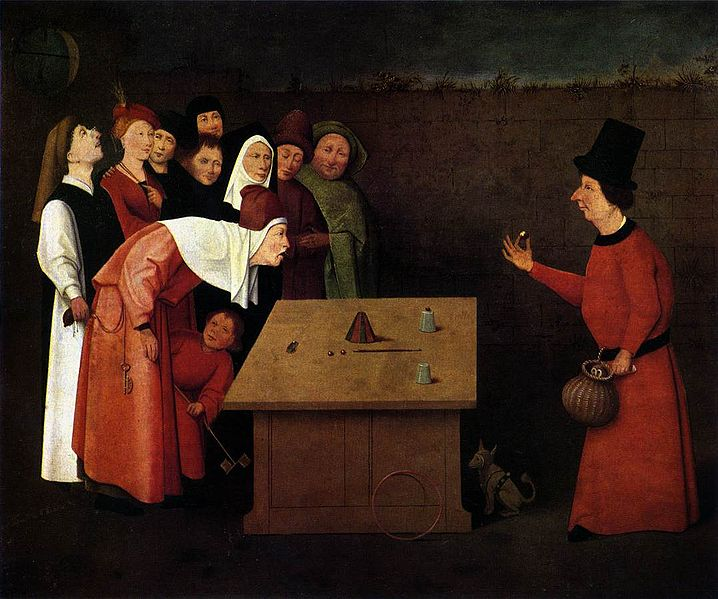
\includegraphics[scale=2.5]{symbolic/2_assembly/718px-Conjurer_Bosch.jpg}
\caption{Hieronymus Bosch -- The Conjurer}
\end{figure}

Again, we can build equivalent function which can take both numerical variables and Expr() objects.
We also extend Expr() class to support many arithmetical and boolean operations.
Also, Expr() methods would take both Expr() objects on input and integer values.

\lstinputlisting{symbolic/2_assembly/1.py}

I run it:

\begin{lstlisting}
((((initial_ECX&65280)|(initial_ECX<<16))<<8)|(((initial_ECX&16711680)|(initial_ECX>>16))>>8))
\end{lstlisting}

Now this is something more readable, however, a bit LISPy at first sight.
In fact, this is a function which change endianness in 32-bit word.

By the way, my Toy Decompiler can do this job as well, but operates on AST (Abstract Syntax Tree) instead
of plain strings: \ref{toy_decompiler}.

\subsubsection{Fast Fourier transform}

I've found one of the smallest possible FFT implementations on \href{https://www.reddit.com/r/Python/comments/1la4jp/understanding_the_fft_algorithm_with_python/}{reddit}:

\lstinputlisting{symbolic/3_FFT/FFT.py}

Just interesting, what value has each element on output?

\lstinputlisting{symbolic/3_FFT/FFT_symb.py}

FFT() function left almost intact, the only thing I added: complex value is converted into string and then
Expr() object is constructed.

\lstinputlisting{symbolic/3_FFT/res1.txt}

We can see subexpressions in form like $x^0$ and $x^1$.
We can eliminate them, since $x^0=1$ and $x^1=x$.
Also, we can reduce subexpressions like $x \cdot 1$ to just $x$.

\begin{lstlisting}
    def __mul__(self, other):
        op1=self.s
        op2=self.convert_to_Expr_if_int(other).s

        if op1=="1":
            return Expr(op2)
        if op2=="1":
            return Expr(op1)

        return Expr("(" + op1 + "*" + op2 + ")")

    def __pow__(self, other):
        op2=self.convert_to_Expr_if_int(other).s
        if op2=="0":
            return Expr("1")
        if op2=="1":
            return Expr(self.s)

        return Expr("(" + self.s + "**" + op2 + ")")
\end{lstlisting}

\lstinputlisting{symbolic/3_FFT/res2.txt}

\subsubsection{Cyclic redundancy check}

I've always been wondering, which input bit affects which bit in the final CRC32 value.

From CRC theory (good and concise introduction:
\url{http://web.archive.org/web/20161220015646/http://www.hackersdelight.org/crc.pdf}
) we know that CRC is shifting register with taps.

We will track each bit rather than byte or word, which is highly inefficient, but serves our purpose better:

\lstinputlisting{symbolic/4_CRC/1.py}

Here are expressions for each CRC32 bit for 1-byte buffer:

\lstinputlisting{symbolic/4_CRC/1byte.txt}

For larger buffer, expressions gets increasing exponentially.
This is 0th bit of the final state for 4-byte buffer:

\begin{lstlisting}
state 0=((((((((((((((in_0_0^1)^(in_0_1^1))^(in_0_2^1))^(in_0_4^1))^(in_0_5^1))^(in_0_7^(1^(in_0_1^1))))^
(in_1_0^(1^(in_0_2^1))))^(in_1_2^(((1^(in_0_0^1))^(in_0_1^1))^(in_0_4^1))))^(in_1_3^(((1^(in_0_1^1))^
(in_0_2^1))^(in_0_5^1))))^(in_1_4^(((1^(in_0_2^1))^(in_0_3^1))^(in_0_6^(1^(in_0_0^1))))))^(in_2_0^((((1^
(in_0_0^1))^(in_0_6^(1^(in_0_0^1))))^(in_0_7^(1^(in_0_1^1))))^(in_1_2^(((1^(in_0_0^1))^(in_0_1^1))^(in_0_4^
1))))))^(in_2_6^(((((((1^(in_0_0^1))^(in_0_1^1))^(in_0_2^1))^(in_0_6^(1^(in_0_0^1))))^(in_1_4^(((1^(in_0_2^1))^
(in_0_3^1))^(in_0_6^(1^(in_0_0^1))))))^(in_1_5^(((1^(in_0_3^1))^(in_0_4^1))^(in_0_7^(1^(in_0_1^1))))))^
(in_2_0^((((1^(in_0_0^1))^(in_0_6^(1^(in_0_0^1))))^(in_0_7^(1^(in_0_1^1))))^(in_1_2^(((1^(in_0_0^1))^(in_0_1^1))^
(in_0_4^1))))))))^(in_2_7^(((((((1^(in_0_1^1))^(in_0_2^1))^(in_0_3^1))^(in_0_7^(1^(in_0_1^1))))^(in_1_5^(((1^
(in_0_3^1))^(in_0_4^1))^(in_0_7^(1^(in_0_1^1))))))^(in_1_6^(((1^(in_0_4^1))^(in_0_5^1))^(in_1_0^(1^(in_0_2^
1))))))^(in_2_1^((((1^(in_0_1^1))^(in_0_7^(1^(in_0_1^1))))^(in_1_0^(1^(in_0_2^1))))^(in_1_3^(((1^(in_0_1^1))^
(in_0_2^1))^(in_0_5^1))))))))^(in_3_2^(((((((((1^(in_0_1^1))^(in_0_2^1))^(in_0_4^1))^(in_0_5^1))^(in_0_6^(1^
(in_0_0^1))))^(in_1_2^(((1^(in_0_0^1))^(in_0_1^1))^(in_0_4^1))))^(in_2_0^((((1^(in_0_0^1))^(in_0_6^(1^(in_0_0^
1))))^(in_0_7^(1^(in_0_1^1))))^(in_1_2^(((1^(in_0_0^1))^(in_0_1^1))^(in_0_4^1))))))^(in_2_1^((((1^(in_0_1^1))^
(in_0_7^(1^(in_0_1^1))))^(in_1_0^(1^(in_0_2^1))))^(in_1_3^(((1^(in_0_1^1))^(in_0_2^1))^(in_0_5^1))))))^(in_2_4^
(((((1^(in_0_0^1))^(in_0_4^1))^(in_1_2^(((1^(in_0_0^1))^(in_0_1^1))^(in_0_4^1))))^(in_1_3^(((1^(in_0_1^1))^
(in_0_2^1))^(in_0_5^1))))^(in_1_6^(((1^(in_0_4^1))^(in_0_5^1))^(in_1_0^(1^(in_0_2^1))))))))))
\end{lstlisting}

Expression for the 0th bit of the final state for 8-byte buffer has length of ~350KiB, which is, of course, can be reduced
significantly (because this expression is basically XOR tree), but you can feel the weight of it.

Now we can process this expressions somehow to get a smaller picture on what is affecting what.
Let's say, if we can find ``in\_2\_3'' substring in expression, this means that 3rd bit of 2nd byte of input
affects this expression.
But even more than that: since this is XOR tree (i.e., expression consisting only of XOR operations),
if some input variable is occurring twice, it's \textit{annihilated}, since $x \oplus x=0$.
More than that: if some vairables occurred even number of times (2, 4, 8, etc), it's annihilated, but left if it's occurred
odd number of times (1, 3, 5, etc).

\begin{lstlisting}
    for i in range(32):
        #print "state %d=%s" % (i, state[31-i])
        sys.stdout.write ("state %02d: " % i)
        for byte in range(BYTES):
            for bit in range(8):
                s="in_%d_%d" % (byte, bit)
                if str(state[31-i]).count(s) & 1:
                    sys.stdout.write ("*")
                else:
                    sys.stdout.write (" ")
        sys.stdout.write ("\n")
\end{lstlisting}

( \url{https://github.com/dennis714/SAT_SMT_article/blob/master/symbolic/4_CRC/2.py} )

Now this how each input bit of 1-byte input buffer affects each bit of the final CRC state:

\lstinputlisting{symbolic/4_CRC/1byte_tbl.txt}

This is 8*8=64 bits of 8-byte input buffer:

\lstinputlisting{symbolic/4_CRC/8byte_tbl.txt}

\subsubsection{Linear congruential generator}

This is popular \ac{PRNG} from OpenWatcom \ac{CRT} library: \url{https://github.com/open-watcom/open-watcom-v2/blob/d468b609ba6ca61eeddad80dd2485e3256fc5261/bld/clib/math/c/rand.c}.

What expression it generates on each step?

\lstinputlisting{symbolic/5_LCG/LCG.py}

\lstinputlisting{symbolic/5_LCG/1.txt}

Now if we once got several values from this PRNG, like 4583, 16304, 14440, 32315, 28670, 12568..., how would we
recover the initial seed?
The problem in fact is solving a system of equations:

\begin{lstlisting}
((((initial_seed*1103515245)+12345)>>16)&32767)==4583
((((((initial_seed*1103515245)+12345)*1103515245)+12345)>>16)&32767)==16304
((((((((initial_seed*1103515245)+12345)*1103515245)+12345)*1103515245)+12345)>>16)&32767)==14440
((((((((((initial_seed*1103515245)+12345)*1103515245)+12345)*1103515245)+12345)*1103515245)+12345)>>16)&32767)==32315
\end{lstlisting}

As it turns out, Z3 can solve this system correctly using only two equations:

\lstinputlisting{symbolic/5_LCG/Z3_solve.py}

\begin{lstlisting}
[x = 11223344]
\end{lstlisting}

(Though, it takes ~20s on my ancient Intel Atom netbook.)

\subsubsection{Path constraint}

How to get weekday from UNIX timestamp?

\begin{lstlisting}
#!/usr/bin/env python

input=...
SECS_DAY=24*60*60
dayno = input / SECS_DAY
wday = (dayno + 4) % 7
if wday==5:
    print "Thanks God, it's Friday!"
\end{lstlisting}

Let's say, we should find a way to run the block with print() call in it.
What input value should be?

First, let's build expression of $wday$ variable:

\lstinputlisting{symbolic/6_TGIF/TGIF.py}

\begin{lstlisting}
(((input/86400)+4)%7)
\end{lstlisting}

In order to execute the block, we should solve this equation: $((\frac{input}{86400}+4) \equiv 5 \mod 7$.

So far, this is easy task for Z3:

\lstinputlisting{symbolic/6_TGIF/Z3_solve.py}

\begin{lstlisting}
[x = 86438]
\end{lstlisting}

This is indeed correct UNIX timestamp for Friday:

\begin{lstlisting}
% date --date='@86438'
Fri Jan  2 03:00:38 MSK 1970
\end{lstlisting}

Though the date back in year 1970, but it's still correct!

This is also called ``path constraint'', i.e., what constraint must be satisified to execute the path into
specific block?
Several tools has ``path'' in their names, like
``pathgrind'', 
\href{http://babelfish.arc.nasa.gov/trac/jpf/wiki/projects/jpf-symbc}{Symbolic PathFinder}, etc.

Like the shell game, this task is also often encounters in practice.
You can see that something dangerous can be executed inside some basic block and you're trying to deduce,
what input values can cause execution of it.
It may be buffer overflow, etc.
Input values are sometimes also called "inputs of death".

Many crackmes are solved in this way, all you need is find a path into block which prints "key is correct"
or something like that.

We can extend this tiny example:

\begin{lstlisting}
input=...
SECS_DAY=24*60*60
dayno = input / SECS_DAY
wday = (dayno + 4) % 7
print wday
if wday==5:
    print "Thanks God, it's Friday!"
else:
    print "Got to wait a little"
\end{lstlisting}

Now we have two blocks: for the first we should solve this equation: $((\frac{input}{86400}+4) \equiv 5 \mod 7$.
But for the second we should solve inverted equation: $((\frac{input}{86400}+4) \not\equiv 5 \mod 7$.
By solving these equations, we will find two paths into both blocks.

KLEE (or similar tool) tries to find path to each [basic] block and produces ``ideal'' unit test.
Hence, KLEE can find a path into the block which crashes everything, or reporting about correctness of the input
key/license, etc.
Surprisingly, KLEE can find backdoors in the very same manner.

KLEE is also called ``KLEE Symbolic Virtual Machine'' -- by that its creators mean that the KLEE is VM which executes a code symbolically rather than numerically.

\subsubsection{Division by zero}

If division by zero is unwrapped and exception isn't caught, it can crash process.

Let's calculate simple expression $\frac{x}{2y + 4z - 12}$.
We can add a warning into \TT{\_\_div\_\_} method:

\lstinputlisting{symbolic/7_div/1.py}

... so it will report about dangerous condition:

\begin{lstlisting}
warning: division by zero if (((y*2)+(z*4))-12)==0
(x/(((y*2)+(z*4))-12))
\end{lstlisting}

This equation is easy to solve, let's try Wolfram Mathematica this time:

\begin{lstlisting}
In[]:= FindInstance[{(y*2 + z*4) - 12 == 0}, {y, z}, Integers]
Out[]= {{y -> 0, z -> 3}}
\end{lstlisting}

These values for $y$ and $z$ can also be called ``inputs of death''.

\subsubsection{Merge sort}

How merge sort works?
I have copypasted Python code from rosettacode.com almost intact:

\lstinputlisting{symbolic/8_sorting/1.py}

But here is a function which compares elements.
Obviously, it wouldn't work correctly without it.

So we can track both expression for each element and numerical value.
Both will be printed finally.
But whenever values are to be compared, only numerical parts will be used.

Result:

\lstinputlisting{symbolic/8_sorting/result.txt}

\subsubsection{Extending Expr class}

This is somewhat senseless, nevertheless, it's easy task to extend my Expr class to support AST trees instead of
plain strings.
It's also possible to add folding steps (like I demonstrated in Toy Decompiler: \ref{toy_decompiler}).
Maybe someone will want to do this as an exercise.

\subsubsection{Conclusion}

For the sake of demonstration, I made things as simple as possible.
But reality is always harsh and inconvenient, so all this shouldn't be taken as a silver bullet.

The files used in this part: \url{https://github.com/dennis714/SAT_SMT_article/tree/master/symbolic}.

As you noticed in my simple examples, expression is represented as a plain string, for the sake of simplicity.
Advanced symbolic execution engines uses \ac{AST}, which are much better and efficient.
\ac{AST} in its simplest form is used in my toy decompiler (\ref{toy_decompiler}).
The toy decompiler can be used as simple symbolic engine as well, just feed all the instructions to it and it will track contents of each register.




\section{KLEE}

% subsections:
\subsection{School-level equation}

Let's revisit school-level system of equations from (\ref{eq2_SMT}).

We will force KLEE to find a path, where all the constraints are satisfied:

\lstinputlisting{KLEE/klee_eq1.c}

% FIXME:
\begin{lstlisting}
% clang -emit-llvm -c -g klee_eq.c
...

% klee klee_eq.bc
KLEE: output directory is "/home/klee/klee-out-93"
KLEE: WARNING: undefined reference to function: klee_assert
KLEE: WARNING ONCE: calling external: klee_assert(0)
KLEE: ERROR: /home/klee/klee_eq.c:18: failed external call: klee_assert
KLEE: NOTE: now ignoring this error at this location

KLEE: done: total instructions = 32
KLEE: done: completed paths = 1
KLEE: done: generated tests = 1
\end{lstlisting}

Let's find out, where \TT{klee\_assert()} has been triggered:

% FIXME:
\begin{lstlisting}
% ls klee-last | grep err
test000001.external.err

% ktest-tool --write-ints klee-last/test000001.ktest
ktest file : 'klee-last/test000001.ktest'
args       : ['klee_eq.bc']
num objects: 3
object    0: name: b'circle'
object    0: size: 4
object    0: data: 5
object    1: name: b'square'
object    1: size: 4
object    1: data: 2
object    2: name: b'triangle'
object    2: size: 4
object    2: data: 1
\end{lstlisting}

This is indeed correct solution to the system of equations.

KLEE has intrinsic \TT{klee\_assume()} which tells KLEE to cut path if some constraint is not true.
So we can rewrite our example in such cleaner way:

\lstinputlisting{KLEE/klee_eq2.c}



\subsection{Zebra puzzle}

Let's revisit zebra puzzle from (\ref{xebra_SMT}).

We just define all variables and add constraints:

\lstinputlisting{KLEE/klee_zebra1.c}

I force KLEE to find distinct values for colors, nationalities, cigarettes, etc, in the same way as I did for Sudoku earlier 
(\ref{sudoku_SMT}).

Let's run it:

% FIXME:
\begin{lstlisting}
% clang -emit-llvm -c -g klee_zebra1.c
...

% klee klee_zebra1.bc
KLEE: output directory is "/home/klee/klee-out-97"
KLEE: WARNING: undefined reference to function: klee_assert
KLEE: WARNING ONCE: calling external: klee_assert(0)
KLEE: ERROR: /home/klee/klee_zebra1.c:130: failed external call: klee_assert
KLEE: NOTE: now ignoring this error at this location

KLEE: done: total instructions = 761
KLEE: done: completed paths = 55
KLEE: done: generated tests = 55
\end{lstlisting}

It works for ~7 seconds on my Intel Core i3-3110M 2.4GHz notebook.
Let's find out path, where \TT{klee\_assert()} has been executed:

% FIXME:
\begin{lstlisting}
% ls klee-last | grep err
test000051.external.err

% ktest-tool --write-ints klee-last/test000051.ktest | less

ktest file : 'klee-last/test000051.ktest'
args       : ['klee_zebra1.bc']
num objects: 25
object    0: name: b'Yellow'
object    0: size: 4
object    0: data: 1
object    1: name: b'Blue'
object    1: size: 4
object    1: data: 2
object    2: name: b'Red'
object    2: size: 4
object    2: data: 3
object    3: name: b'Ivory'
object    3: size: 4
object    3: data: 4

...

object   21: name: b'Horse'
object   21: size: 4
object   21: data: 2
object   22: name: b'Snails'
object   22: size: 4
object   22: data: 3
object   23: name: b'Dog'
object   23: size: 4
object   23: data: 4
object   24: name: b'Zebra'
object   24: size: 4
object   24: data: 5
\end{lstlisting}

This is indeed correct solution.

\TT{klee\_assume()} also can be used this time:

\lstinputlisting{KLEE/klee_zebra2.c}

\dots and this version works slightly faster ($\approx 5$ seconds),
maybe because KLEE is aware of this intrinsic and handles it in a special way?


\subsection{Sudoku}

I've also rewritten Sudoku example (XXX) for KLEE: % FIXME \ref{}

\lstinputlisting[numbers=left]{KLEE/klee_sudoku_or1.c}

Let's run it:

% FIXME:
\begin{lstlisting}
\$ clang -emit-llvm -c -g klee_sudoku_or1.c
...

\$ time klee klee_sudoku_or1.bc
KLEE: output directory is "/home/klee/klee-out-98"
KLEE: WARNING: undefined reference to function: klee_assert
KLEE: WARNING ONCE: calling external: klee_assert(0)
KLEE: ERROR: /home/klee/klee_sudoku_or1.c:93: failed external call: klee_assert
KLEE: NOTE: now ignoring this error at this location

KLEE: done: total instructions = 7512
KLEE: done: completed paths = 161
KLEE: done: generated tests = 161

real    3m44.111s
user    3m43.319s
sys     0m0.951s
\end{lstlisting}

Now this is really slower (on my XXX) in comparison to Z3Py solution (XXX). % FIXME \ref{}

But the answer is correct:

% FIXME:
\begin{lstlisting}
\$ ls klee-last | grep err
test000161.external.err

\$ ktest-tool --write-ints klee-last/test000161.ktest
ktest file : 'klee-last/test000161.ktest'
args       : ['klee_sudoku_or1.bc']
num objects: 1
object    0: name: b'cells'
object    0: size: 81
object    0: data: b'\x01\x04\x05\x03\x02\x07\x06\t\x08\x08\x03\t\x06\x05\x04\x01\x02\x07\x06\x07\x02\t\x01\x08\x05\x04\x03\x04\t\x06\x01\x08\x05\x03\x07\x02\x02\x01\x08\x04\x07\x03\t\x05\x06\x07\x05\x03\x02\t\x06\x04\x08\x01\x03\x06\x07\x05\x04\x02\x08\x01\t\t\x08\x04\x07\x06\x01\x02\x03\x05\x05\x02\x01\x08\x03\t\x07\x06\x04'
\end{lstlisting}

% FIXME backslash
\TT{\\t} is character with ASCII code of 9 in C/C++, and KLEE attempts to treat byte array as C/C++ string, so it shows some values in such way.
We can just remember that there is 9 at the each place where we see \TT{\\t}.
The solution, while not properly formatted, correct indeed (XXX).\\ % FIXME \ref{}
\\
By the way, at lines 42, 43 you may see how we tell to KLEE that all array elements must be within some limits.
If we comment these lines out, we've got this:

% FIXME:
\begin{lstlisting}
\$ time klee klee_sudoku_or1.bc
KLEE: output directory is "/home/klee/klee-out-100"
KLEE: WARNING: undefined reference to function: klee_assert
KLEE: ERROR: /home/klee/klee_sudoku_or1.c:51: overshift error
KLEE: NOTE: now ignoring this error at this location
KLEE: ERROR: /home/klee/klee_sudoku_or1.c:51: overshift error
KLEE: NOTE: now ignoring this error at this location
KLEE: ERROR: /home/klee/klee_sudoku_or1.c:51: overshift error
KLEE: NOTE: now ignoring this error at this location
...
\end{lstlisting}

KLEE warns us that shift value at line 51 is too big.
Indeed, KLEE may try all byte values up to 255 (0xFF), which are pointless to use there, and may indicate error or bug, so KLEE warns about it.\\
\\
Now let's use \TT{klee\_assume()} again:

\lstinputlisting{KLEE/klee_sudoku_or2.c}

% FIXME:
\begin{lstlisting}
\$ time klee klee_sudoku_or2.bc
KLEE: output directory is "/home/klee/klee-out-99"
KLEE: WARNING: undefined reference to function: klee_assert
KLEE: WARNING ONCE: calling external: klee_assert(0)
KLEE: ERROR: /home/klee/klee_sudoku_or2.c:93: failed external call: klee_assert
KLEE: NOTE: now ignoring this error at this location

KLEE: done: total instructions = 7119
KLEE: done: completed paths = 1
KLEE: done: generated tests = 1

real    0m35.312s
user    0m34.945s
sys     0m0.318s
\end{lstlisting}

That works much faster: perhaps KLEE indeed handle this intrinsic in a special way.
And, as we see, the only one path is generated (one we actually interesting in it) instead of 161.

It's still much slower than Z3Py solution, though.


\subsection{Unit test: HTML color}

The most popular ways to represent HTML/CSS color is by English name (e.g., ``red'') and by 6-digit hexadecimal number (e.g., ``\#0077CC'').
There is third, less popular way: if each byte in hexadecimal number has two doubling digits, it can be \textit{abbreviated}, thus, 
``\#0077CC'' can be written just as ``\#07C''.

Let's write a function to convert 3 color components into name (if possible, first priority), 3-digit hexadecimal form (if possible, second priority),
or as 6-digit hexadecimal form (as a last resort).

\lstinputlisting{KLEE/color.c}

There are 5 paths in function, and let's see, if KLEE could find them all?
It's indeed so:

% FIXME:
\begin{lstlisting}
% clang -emit-llvm -c -g color.c

% klee color.bc
KLEE: output directory is "/home/klee/klee-out-134"
KLEE: WARNING: undefined reference to function: sprintf
KLEE: WARNING: undefined reference to function: strcpy
KLEE: WARNING ONCE: calling external: strcpy(51867584, 51598960)
KLEE: ERROR: /home/klee/color.c:33: external call with symbolic argument: sprintf
KLEE: NOTE: now ignoring this error at this location
KLEE: ERROR: /home/klee/color.c:28: external call with symbolic argument: sprintf
KLEE: NOTE: now ignoring this error at this location

KLEE: done: total instructions = 479
KLEE: done: completed paths = 19
KLEE: done: generated tests = 5
\end{lstlisting}

We can ignore calls to strcpy() and sprintf(), because we are not really interesting in state of \TT{out} variable.

So there are exactly 5 paths:

% FIXME:
\begin{lstlisting}
% ls klee-last
assembly.ll   run.stats            test000003.ktest     test000005.ktest
info          test000001.ktest     test000003.pc        test000005.pc
messages.txt  test000002.ktest     test000004.ktest     warnings.txt
run.istats    test000003.exec.err  test000005.exec.err
\end{lstlisting}

1st set of input variables will result in ``red'' string:

% FIXME:
\begin{lstlisting}
% ktest-tool --write-ints klee-last/test000001.ktest
ktest file : 'klee-last/test000001.ktest'
args       : ['color.bc']
num objects: 3
object    0: name: b'R'
object    0: size: 1
object    0: data: b'\xff'
object    1: name: b'G'
object    1: size: 1
object    1: data: b'\x00'
object    2: name: b'B'
object    2: size: 1
object    2: data: b'\x00'
\end{lstlisting}

2nd set of input variables will result in ``green'' string:

% FIXME:
\begin{lstlisting}
% ktest-tool --write-ints klee-last/test000002.ktest
ktest file : 'klee-last/test000002.ktest'
args       : ['color.bc']
num objects: 3
object    0: name: b'R'
object    0: size: 1
object    0: data: b'\x00'
object    1: name: b'G'
object    1: size: 1
object    1: data: b'\xff'
object    2: name: b'B'
object    2: size: 1
object    2: data: b'\x00'
\end{lstlisting}

3rd set of input variables will result in ``\#010000'' string:

% FIXME:
\begin{lstlisting}
% ktest-tool --write-ints klee-last/test000003.ktest
ktest file : 'klee-last/test000003.ktest'
args       : ['color.bc']
num objects: 3
object    0: name: b'R'
object    0: size: 1
object    0: data: b'\x01'
object    1: name: b'G'
object    1: size: 1
object    1: data: b'\x00'
object    2: name: b'B'
object    2: size: 1
object    2: data: b'\x00'
\end{lstlisting}

4th set of input variables will result in ``blue'' string:

% FIXME:
\begin{lstlisting}
% ktest-tool --write-ints klee-last/test000004.ktest
ktest file : 'klee-last/test000004.ktest'
args       : ['color.bc']
num objects: 3
object    0: name: b'R'
object    0: size: 1
object    0: data: b'\x00'
object    1: name: b'G'
object    1: size: 1
object    1: data: b'\x00'
object    2: name: b'B'
object    2: size: 1
object    2: data: b'\xff'
\end{lstlisting}

5th set of input variables will result in ``\#F01'' string:

% FIXME:
\begin{lstlisting}
% ktest-tool --write-ints klee-last/test000005.ktest
ktest file : 'klee-last/test000005.ktest'
args       : ['color.bc']
num objects: 3
object    0: name: b'R'
object    0: size: 1
object    0: data: b'\xff'
object    1: name: b'G'
object    1: size: 1
object    1: data: b'\x00'
object    2: name: b'B'
object    2: size: 1
object    2: data: b'\x11'
\end{lstlisting}

These 5 sets of input variables can form a unit test for our function.


\subsection{Unit test: strcmp() function}

The standard \TT{strcmp()} function from C library can return 0, -1 and 1, depending of comparison result.

Here is my own implementation of strcmp():

\lstinputlisting{KLEE/strcmp.c}

Let's find out, if KLEE is capable of finding all three paths?
I intentionaly made things simpler for KLEE by limiting input arrays to two 2 bytes or to 1 character + terminal zero byte.

% FIXME:
\begin{lstlisting}[basicstyle=\ttfamily, mathescape]
$\$$ clang -emit-llvm -c -g strcmp.c

$\$$ klee strcmp.bc
KLEE: output directory is "/home/klee/klee-out-131"
KLEE: ERROR: /home/klee/strcmp.c:35: invalid klee_assume call (provably false)
KLEE: NOTE: now ignoring this error at this location
KLEE: ERROR: /home/klee/strcmp.c:36: invalid klee_assume call (provably false)
KLEE: NOTE: now ignoring this error at this location

KLEE: done: total instructions = 137
KLEE: done: completed paths = 5
KLEE: done: generated tests = 5

$\$$ ls klee-last
assembly.ll   run.stats            test000002.ktest     test000004.ktest
info          test000001.ktest     test000002.pc        test000005.ktest
messages.txt  test000001.pc        test000002.user.err  warnings.txt
run.istats    test000001.user.err  test000003.ktest
\end{lstlisting}

The first two errors are about klee\_assume().
These are input values on which klee\_assume() calls are stuck.
We can ignore them, or take a peek out of curiosity:

% FIXME:
\begin{lstlisting}
\$ ktest-tool --write-ints klee-last/test000001.ktest
ktest file : 'klee-last/test000001.ktest'
args       : ['strcmp.bc']
num objects: 2
object    0: name: b'input1'
object    0: size: 2
object    0: data: b'\x00\x00'
object    1: name: b'input2'
object    1: size: 2
object    1: data: b'\x00\x00'

\$ ktest-tool --write-ints klee-last/test000002.ktest
ktest file : 'klee-last/test000002.ktest'
args       : ['strcmp.bc']
num objects: 2
object    0: name: b'input1'
object    0: size: 2
object    0: data: b'a\xff'
object    1: name: b'input2'
object    1: size: 2
object    1: data: b'\x00\x00'
\end{lstlisting}

Three rest files are the input values for each path inside of my implementation of strcmp():

% FIXME:
\begin{lstlisting}
\$ ktest-tool --write-ints klee-last/test000003.ktest
ktest file : 'klee-last/test000003.ktest'
args       : ['strcmp.bc']
num objects: 2
object    0: name: b'input1'
object    0: size: 2
object    0: data: b'b\x00'
object    1: name: b'input2'
object    1: size: 2
object    1: data: b'c\x00'

\$ ktest-tool --write-ints klee-last/test000004.ktest
ktest file : 'klee-last/test000004.ktest'
args       : ['strcmp.bc']
num objects: 2
object    0: name: b'input1'
object    0: size: 2
object    0: data: b'c\x00'
object    1: name: b'input2'
object    1: size: 2
object    1: data: b'a\x00'

\$ ktest-tool --write-ints klee-last/test000005.ktest
ktest file : 'klee-last/test000005.ktest'
args       : ['strcmp.bc']
num objects: 2
object    0: name: b'input1'
object    0: size: 2
object    0: data: b'a\x00'
object    1: name: b'input2'
object    1: size: 2
object    1: data: b'a\x00'
\end{lstlisting}

3rd is about first argument (``b'') is lesser than the second (``c'').
4th is opposite (``c'' and ``a'').
5th is when they are equal (``a'' and ``a'').\\
\\
Using these 3 test cases, we've got full coverage of our implementation of strcmp().


\subsection{UNIX date/time}

UNIX date/time\footnote{\url{https://en.wikipedia.org/wiki/Unix_time}} is a number of seconds that have elapsed since 1-Jan-1970 00:00 UTC.
C/C++ gmtime() function is used to decode this value into human-readable date/time.

Here is a piece of code I've copypasted from some ancient version of Minix OS 
(\url{http://www.cise.ufl.edu/~cop4600/cgi-bin/lxr/http/source.cgi/lib/ansi/gmtime.c}) and reworked slightly:

\lstinputlisting[numbers=left]{KLEE/klee_time1.c}

Let's try it:

% FIXME:
\begin{lstlisting}
\$ clang -emit-llvm -c -g klee_time1.c
...

\$ klee klee_time1.bc
KLEE: output directory is "/home/klee/klee-out-107"
KLEE: WARNING: undefined reference to function: printf
KLEE: ERROR: /home/klee/klee_time1.c:86: external call with symbolic argument: printf
KLEE: NOTE: now ignoring this error at this location
KLEE: ERROR: /home/klee/klee_time1.c:83: ASSERTION FAIL: 0
KLEE: NOTE: now ignoring this error at this location

KLEE: done: total instructions = 101579
KLEE: done: completed paths = 1635
KLEE: done: generated tests = 2
\end{lstlisting}

Wow, assert() at line 83 has been triggered, why?
Let's see a value of UNIX time which triggers it:

% FIXME:
\begin{lstlisting}
\$ ls klee-last | grep err
test000001.exec.err
test000002.assert.err

\$ ktest-tool --write-ints klee-last/test000002.ktest
ktest file : 'klee-last/test000002.ktest'
args       : ['klee_time1.bc']
num objects: 1
object    0: name: b'time'
object    0: size: 4
object    0: data: 978278400
\end{lstlisting}

Let's decode this value using UNIX date utility:

% FIXME:
\begin{lstlisting}
\$ date -u --date='@978278400'
Sun Dec 31 16:00:00 UTC 2000
\end{lstlisting}

After may investigation, I've found that \TT{month} variable can hold incorrect value of 12 (while 11 is maximal, for December), 
because LEAPYEAR() macro should receive year number as 2000, not as 100.
So I've introduced a bug during rewritting this function, and KLEE found it!

Just interesting, what would be if I'll replace switch() to array of strings, like it usually happens in concise C/C++ code?

% FIXME:
\begin{lstlisting}
	...

const char *_months[] =
{
	"January", "February", "March",
	"April", "May", "June",
	"July", "August", "September",
	"October", "November", "December"
};

	...

	while (dayno >= _ytab[LEAPYEAR(year)][month])
	{
		dayno -= _ytab[LEAPYEAR(year)][month];
		month++;
	}
	
	char *s=_months[month];

	printf ("%04d-%s-%02d %02d:%02d:%02d\n", YEAR0+year, s, dayno+1, hour, minutes, seconds);
	printf ("week day: %s\n", _days[wday]);	
	
	...

\end{lstlisting}

KLEE detects attempt to read beyond array boundaries:

% FIXME:
\begin{lstlisting}
\$ klee klee_time2.bc
KLEE: output directory is "/home/klee/klee-out-108"
KLEE: WARNING: undefined reference to function: printf
KLEE: ERROR: /home/klee/klee_time2.c:69: external call with symbolic argument: printf
KLEE: NOTE: now ignoring this error at this location
KLEE: ERROR: /home/klee/klee_time2.c:67: memory error: out of bound pointer
KLEE: NOTE: now ignoring this error at this location

KLEE: done: total instructions = 101716
KLEE: done: completed paths = 1635
KLEE: done: generated tests = 2
\end{lstlisting}

This is the same UNIX time value we've already seen:

% FIXME:
\begin{lstlisting}
\$ ls klee-last | grep err
test000001.exec.err
test000002.ptr.err

\$ ktest-tool --write-ints klee-last/test000002.ktest
ktest file : 'klee-last/test000002.ktest'
args       : ['klee_time2.bc']
num objects: 1
object    0: name: b'time'
object    0: size: 4
object    0: data: 978278400
\end{lstlisting}

So, if this piece of code can be triggered on remote computer, with this input value (\textit{input of death}),
it's possible to crash the process (with some luck, though).\\
\\
OK, now I'm fixing a bug by moving year subtracting expression to line 43, and let's find, what UNIX time value corresponds to some fancy date
like 2022-February-2?

\lstinputlisting[numbers=left]{KLEE/klee_time3.c}

% FIXME:
\begin{lstlisting}
\$ clang -emit-llvm -c -g klee_time3.c
...

\$ klee klee_time3.bc
KLEE: output directory is "/home/klee/klee-out-109"
KLEE: WARNING: undefined reference to function: klee_assert
KLEE: WARNING ONCE: calling external: klee_assert(0)
KLEE: ERROR: /home/klee/klee_time3.c:47: failed external call: klee_assert
KLEE: NOTE: now ignoring this error at this location

KLEE: done: total instructions = 101087
KLEE: done: completed paths = 1635
KLEE: done: generated tests = 1635

\$ ls klee-last | grep err
test000587.external.err

\$ ktest-tool --write-ints klee-last/test000587.ktest
ktest file : 'klee-last/test000587.ktest'
args       : ['klee_time3.bc']
num objects: 1
object    0: name: b'time'
object    0: size: 4
object    0: data: 1645488640

\$ date -u --date='@1645488640'
Tue Feb 22 00:10:40 UTC 2022
\end{lstlisting}

Success, but hours/minutes/seconds are seems random -- they are random indeed, because, KLEE satisfied all constraints we've put, nothing else.
We didn't ask it to set hours/minutes/seconds to zeroes.

Let's add constraints to hours/minutes/seconds as well:

% FIXME:
\begin{lstlisting}
	...

	if (YEAR0+year==2022 && month==1 && dayno+1==22 && hour==22 && minutes==22 && seconds==22)
		klee_assert(0);
	
	...
\end{lstlisting}

Let's run it and check...

% FIXME:
\begin{lstlisting}
\$ ktest-tool --write-ints klee-last/test000597.ktest
ktest file : 'klee-last/test000597.ktest'
args       : ['klee_time3.bc']
num objects: 1
object    0: name: b'time'
object    0: size: 4
object    0: data: 1645568542

\$ date -u --date='@1645568542'
Tue Feb 22 22:22:22 UTC 2022
\end{lstlisting}

Now that is precise.

Yes, of course, C/C++ libraries has function(s) to encode human-readable date into UNIX time value, but what we've got here is KLEE working
\textit{antipode} of decoding function, \textit{inverse function} in a way.


\subsection{Inverse function for base64 decoder}

It's piece of cake for KLEE to reconstruct input base64 string given just base64 decoder without encoder.
I've copypasted this piece of code somewhere.

We add constraints (lines 84, 85) so that output buffer must have byte values from 0 to 15.
We also tell to KLEE that the Base64decode() function must return 16 (i.e., size of output buffer in bytes, line 82).

\lstinputlisting[numbers=left]{KLEE/klee_base64.c}

% FIXME:
\begin{lstlisting}
\$ clang -emit-llvm -c -g klee_base64.c
...

\$ klee klee_base64.bc
KLEE: output directory is "/home/klee/klee-out-99"
KLEE: WARNING: undefined reference to function: klee_assert
KLEE: ERROR: /home/klee/klee_base64.c:99: invalid klee_assume call (provably false)
KLEE: NOTE: now ignoring this error at this location
KLEE: WARNING ONCE: calling external: klee_assert(0)
KLEE: ERROR: /home/klee/klee_base64.c:104: failed external call: klee_assert
KLEE: NOTE: now ignoring this error at this location
KLEE: ERROR: /home/klee/klee_base64.c:85: memory error: out of bound pointer
KLEE: NOTE: now ignoring this error at this location
KLEE: ERROR: /home/klee/klee_base64.c:81: memory error: out of bound pointer
KLEE: NOTE: now ignoring this error at this location
KLEE: ERROR: /home/klee/klee_base64.c:65: memory error: out of bound pointer
KLEE: NOTE: now ignoring this error at this location

...
\end{lstlisting}

We're interesting in the second error, where \TT{klee\_assert()} has been triggered:

% FIXME:
\begin{lstlisting}
\$ ls klee-last | grep err
test000001.user.err
test000002.external.err
test000003.ptr.err
test000004.ptr.err
test000005.ptr.err

\$ ktest-tool --write-ints klee-last/test000002.ktest
ktest file : 'klee-last/test000002.ktest'
args       : ['klee_base64.bc']
num objects: 1
object    0: name: b'input'
object    0: size: 32
object    0: data: b'AAECAwQFBgcICQoLDA0OD4\x00\xff\xff\xff\xff\xff\xff\xff\xff\x00'
\end{lstlisting}

This is indeed a real base64 string, terminated with the zero byte, just as it's requested by C/C++ standards.
The final zero byte at 31th byte (starting at zeroth byte) is our deed: so that KLEE would report lesser number of errors. % FIXME spelling

The base64 string is indeed correct:

% FIXME:
\begin{lstlisting}
\$ echo AAECAwQFBgcICQoLDA0OD4 | base64 -d | hexdump -C
base64: invalid input
00000000  00 01 02 03 04 05 06 07  08 09 0a 0b 0c 0d 0e 0f  |................|
00000010
\end{lstlisting}

base64 decoder Linux utility I've just run blaming for ``invalid input'' -- it means input string is not properly padded:
Now let's pad it manually, and decoder utility will no complain anymore:

% FIXME:
\begin{lstlisting}
\$ echo AAECAwQFBgcICQoLDA0OD4== | base64 -d | hexdump -C
00000000  00 01 02 03 04 05 06 07  08 09 0a 0b 0c 0d 0e 0f  |................|
00000010
\end{lstlisting}

The reason our generated base64 string is not padded is because base64 decoders are usually discards padding symbols (``='') at the end.
In other words, they are not require them, so is the case of our decoder.
Padding symbols are left unnoticed to KLEE.

So we again made \textit{antipode} or \textit{inverse function} of base64 decoder.


\subsection{CRC} % FIXME full name

\subsubsection{Buffer alteration case \#1}

Sometimes, you need to alter a piece of data which is \textit{protected} by some kind of checksum or \ac{CRC}, and you can't change checksum or CRC value, but can alter piece of data so that checksum will remain the same.

Let's pretend, we've got a piece of data with ``Hello, world!'' string at the beginning and ``and goodbye'' string at the end.
We can alter 14 characters at the middle, but for some reason, they must be in \textit{a..z} limits, but we can put any characters there.
CRC64 of the whole block must be \TT{0x12345678abcdef12}.

Let's see\footnote{There are several slightly different CRC64 implementations, the one I use here can also be different from popular ones.}:

\lstinputlisting{KLEE/klee_CRC64.c}

Since our code uses memcmp() standard C/C++ function, we need to add \TT{--libc=uclibc} switch, so KLEE will use its own uClibc % FIXME check spelling
implementation. % \ref{} -> closed programs

% FIXME:
\begin{lstlisting}
% clang -emit-llvm -c -g klee_CRC64.c

% time klee --libc=uclibc klee_CRC64.bc
\end{lstlisting}

It takes about 1 minute (on my Intel Core i3-3110M 2.4GHz notebook) and we getting this:

% FIXME:
\begin{lstlisting}
...
real    0m52.643s
user    0m51.232s
sys     0m0.239s
...
\$ ls klee-last | grep err
test000001.user.err
test000002.user.err
test000003.user.err
test000004.external.err

\$ ktest-tool --write-ints klee-last/test000004.ktest
ktest file : 'klee-last/test000004.ktest'
args       : ['klee_CRC64.bc']
num objects: 1
object    0: name: b'buf'
object    0: size: 46
object    0: data: b'Hello, world!.. qqlicayzceamyw ... and goodbye'
\end{lstlisting}

Maybe it's slow, but definitely faster than bruteforce.
Indeed, $log_2{26^{14}} \approx 65.8$
which is close to 64 bits.
In other words, one need $\approx 14$ latin characters to encode 64 bits.
And KLEE + \ac{SMT} solver needs 64 bits at some place it can alter to make final CRC64 value equal to what we defined.

I tried to reduce length of the \textit{middle block} to 13 characters: no luck for KLEE then, it has no space enough.

\subsubsection{Buffer alteration case \#2}

I went sadistic: what if the buffer must contain the CRC64 value which, after calculation of CRC64, will result in the same value?
Fascinately, % FIXME check spelling
KLEE can solve this.
The buffer will have the following format:

% FIXME:
\begin{lstlisting}
Hello, world! <8-bytes (64-bit value)> and goodbye <6 more bytes>
\end{lstlisting}

% FIXME:
\begin{lstlisting}
int main()
{
#define HEAD_STR "Hello, world!.. "
#define HEAD_SIZE strlen(HEAD_STR)
#define TAIL_STR " ... and goodbye"
#define TAIL_SIZE strlen(TAIL_STR)
// 8 bytes for 64-bit value:
#define MID_SIZE 8
#define BUF_SIZE HEAD_SIZE+TAIL_SIZE+MID_SIZE+6

	char buf[BUF_SIZE];
  
	klee_make_symbolic(buf, sizeof buf, "buf");

	klee_assume (memcmp (buf, HEAD_STR, HEAD_SIZE)==0);

	klee_assume (memcmp (buf+HEAD_SIZE+MID_SIZE, TAIL_STR, TAIL_SIZE)==0);
	
	uint64_t mid_value=*(uint64_t*)(buf+HEAD_SIZE);
	klee_assume (crc64 (0, buf, BUF_SIZE)==mid_value);

	klee_assert(0);

	return 0;
}
\end{lstlisting}

It works:

% FIXME:
\begin{lstlisting}
% time klee --libc=uclibc klee_CRC64.bc
...
real    5m17.081s
user    5m17.014s
sys     0m0.319s

% ls klee-last | grep err
test000001.user.err
test000002.user.err
test000003.external.err

% ktest-tool --write-ints klee-last/test000003.ktest
ktest file : 'klee-last/test000003.ktest'
args       : ['klee_CRC64.bc']
num objects: 1
object    0: name: b'buf'
object    0: size: 46
object    0: data: b'Hello, world!.. T+]\xb9A\x08\x0fq ... and goodbye\xb6\x8f\x9c\xd8\xc5\x00'
\end{lstlisting}

8 bytes between two strings is 64-bit value which equals to CRC64 of this whole block.
Again, it's faster than brute-force way to find it.
If to decrease last spare 6-byte buffer to 4 bytes or less, KLEE works so long so I've stopped it.

\subsubsection{Recovering input data for given CRC32 value of it}

I've always wanted to do so, but everyone knows this is impossible for input buffers larger than 4 bytes.
As my experiments show, it's still possible for tiny input buffers of data, constrained in some way.

The CRC32 value of 6-byte ``SILVER'' string is known: \TT{0xDFA3DFDD}.
KLEE can find this 6-byte string, if it knows that each byte of input buffer is in \textit{A..Z} limits:

\lstinputlisting[numbers=left]{KLEE/klee_SILVER.c}

% FIXME:
\begin{lstlisting}
% clang -emit-llvm -c -g klee_SILVER.c
...

% klee klee_SILVER.bc
...

% ls klee-last | grep err
test000013.external.err

\$ ktest-tool --write-ints klee-last/test000013.ktest
ktest file : 'klee-last/test000013.ktest'
args       : ['klee_SILVER.bc']
num objects: 1
object    0: name: b'str'
object    0: size: 6
object    0: data: b'SILVER'
\end{lstlisting}

Still, it's no magic: if to remove condition at lines 23..25 (i.e., if to relax constraints),
KLEE will produce some other string, which will be still correct for the CRC32 value given.

It works, because 6 Latin characters in \textit{A..Z} limits contain $\approx 28.2$ bits:
$log_2{26^6} \approx 28.2$, which is even smaller value than 32.
In other words, the final CRC32 value holds enough bits to recover $\approx 28.2$ bits of input.

The input buffer can be even bigger, if each byte of it will be in even tighter % FIXME spelling
constraints (decimal digits, binary digits, etc).

\subsubsection{In comparison with other hashing algorithms}

Things are that easy for some other hashing algorithms like \textit{fletcher checksum}, % FIXME URL
but not for cryptographically secure ones (like MD5, SHA1, etc), they are protected from such simple cryptoanalysis. % FIXME \ref{} -> am.crypto


\subsection{LZSS decompressor}

I've googled for a very simple LZSS decompressor and landed at this page:
\url{http://www.opensource.apple.com/source/boot/boot-132/i386/boot2/lzss.c}.

Let's pretend, we're looking at unknown compressing algorithm with no compressor available.
Will it be possible to construct a compressed piece of data so that decompressor would generate data we need?

Here is my first experiment:

\lstinputlisting{KLEE/klee_lzss1.c}

What I did is changing size of ring buffer from 4096 to 32, because if bigger, KLEE consumes all RAM it can.
I found that KLEE can live with that small buffer.
I also decreased \TT{COMPRESSED\_LEN} gradually to check, whether KLEE would find compressed piece of data, and it did:

% FIXME:
\begin{lstlisting}
\$ clang -emit-llvm -c -g klee_lzss.c
...

\$ time klee klee_lzss.bc
KLEE: output directory is "/home/klee/klee-out-7"
KLEE: WARNING: undefined reference to function: klee_assert
KLEE: ERROR: /home/klee/klee_lzss.c:122: invalid klee_assume call (provably false)
KLEE: NOTE: now ignoring this error at this location
KLEE: ERROR: /home/klee/klee_lzss.c:47: memory error: out of bound pointer
KLEE: NOTE: now ignoring this error at this location
KLEE: ERROR: /home/klee/klee_lzss.c:37: memory error: out of bound pointer
KLEE: NOTE: now ignoring this error at this location
KLEE: WARNING ONCE: calling external: klee_assert(0)
KLEE: ERROR: /home/klee/klee_lzss.c:124: failed external call: klee_assert
KLEE: NOTE: now ignoring this error at this location

KLEE: done: total instructions = 41417919
KLEE: done: completed paths = 437820
KLEE: done: generated tests = 4

real    13m0.215s
user    11m57.517s
sys     1m2.187s

\$ ls klee-last | grep err
test000001.user.err
test000002.ptr.err
test000003.ptr.err
test000004.external.err

\$ ktest-tool --write-ints klee-last/test000004.ktest
ktest file : 'klee-last/test000004.ktest'
args       : ['klee_lzss.bc']
num objects: 1
object    0: name: b'input'
object    0: size: 15
object    0: data: b'\xffBuffalo \x01b\x0f\x03\r\x05'
\end{lstlisting}

% FIXME tilde
KLEE consumed ~1GB of RAM and worked for ~15 minutes (on my Intel Core i3-3110M 2.4GHz notebook), 
but here it is, a 15 bytes which, if decompressed by our copypasted algorithm, will result in desired text!

During my experimentation, I've found that KLEE can do even more cooler thing, to find out size of compressed piece of data:

% FIXME:
\begin{lstlisting}
int main()
{
	uint8_t input[24];
	uint8_t plain[24];
	uint32_t size;
  
	klee_make_symbolic(input, sizeof input, "input");
	klee_make_symbolic(&size, sizeof size, "size");
	
	decompress_lzss(plain, input, size);

	for (int i=0; i<23; i++)
		klee_assume (plain[i]=="Buffalo buffalo Buffalo"[i]);

	klee_assert(0);
	
	return 0;
}
\end{lstlisting}

... but then KLEE works much slower, consumes much more RAM and I had success only with even smaller pieces of desired text.

So how LZSS works? Without peeking into Wikipedia, we can say that: 
if LZSS compressor observes some data it already had, it replaces the data with a link to some place in past with size. 
If it observes something yet unseen, it puts data as is.
This is theory.
This is indeed what we've got. Desired text is three ``Buffalo'' words, the first and the last are equivalent, but the second is \textit{almost} equivalent, 
differing with first by one character.

That's what we see:

% FIXME: colored Buffalo, ``b'', slashes
\begin{lstlisting}
'\xffBuffalo \x01b\x0f\x03\r\x05'
\end{lstlisting}

Here is some control byte (0xff), ``Buffalo'' word is placed \textit{as is}, then another control byte (0x01), 
then we see beginning of the second word (``b'') and more
control bytes, perhaps, links to the beginning of the buffer.
These are command to decompressor, like, in plain English, ``copy data from the buffer we've already done, from that place to that place'', etc.

Interesting, is it possible to meddle into this piece of compressed data?
Out of whim, can we force KLEE to find a compressed data, where not just ``b'' character has been placed \textit{as is},
but also the second character of the word, i.e., ``bu''?

I've modified main() function by adding \TT{klee\_assume()}: now the 11th byte of input (compressed) data (right after ``b'' byte) should have ``u''.
I has no luck with 15 byte of compressed data, so I increased it to 16 bytes:

% FIXME:
\begin{lstlisting}
int main()
{
#define COMPRESSED_LEN 16
	uint8_t input[COMPRESSED_LEN];
	uint8_t plain[24];
	uint32_t size=COMPRESSED_LEN;
  
	klee_make_symbolic(input, sizeof input, "input");
	
	klee_assume(input[11]=='u');
	
	decompress_lzss(plain, input, size);

	for (int i=0; i<23; i++)
		klee_assume (plain[i]=="Buffalo buffalo Buffalo"[i]);

	klee_assert(0);
	
	return 0;
}
\end{lstlisting}

% FIXME: umlaut
... and voila: KLEE found a compressed piece of data which satisfied our whimsical constraint:

% FIXME:
\begin{lstlisting}
\$ time klee klee_lzss.bc
KLEE: output directory is "/home/klee/klee-out-9"
KLEE: WARNING: undefined reference to function: klee_assert
KLEE: ERROR: /home/klee/klee_lzss.c:97: invalid klee_assume call (provably false)
KLEE: NOTE: now ignoring this error at this location
KLEE: ERROR: /home/klee/klee_lzss.c:47: memory error: out of bound pointer
KLEE: NOTE: now ignoring this error at this location
KLEE: ERROR: /home/klee/klee_lzss.c:37: memory error: out of bound pointer
KLEE: NOTE: now ignoring this error at this location
KLEE: WARNING ONCE: calling external: klee_assert(0)
KLEE: ERROR: /home/klee/klee_lzss.c:99: failed external call: klee_assert
KLEE: NOTE: now ignoring this error at this location

KLEE: done: total instructions = 36700587
KLEE: done: completed paths = 369756
KLEE: done: generated tests = 4

real    12m16.983s
user    11m17.492s
sys     0m58.358s

\$ ktest-tool --write-ints klee-last/test000004.ktest
ktest file : 'klee-last/test000004.ktest'
args       : ['klee_lzss.bc']
num objects: 1
object    0: name: b'input'
object    0: size: 16
object    0: data: b'\xffBuffalo \x13bu\x10\x02\r\x05'
\end{lstlisting}

So now we find a piece of data where two strings are placed \textit{as is}: ``Buffalo'' and ``bu''.

% FIXME: colored Buffalo and bu
\begin{lstlisting}
'\xffBuffalo \x13bu\x10\x02\r\x05'
\end{lstlisting}

Both pieces of compressed data, if feeded into our copypasted function, produce ``Buffalo buffalo Buffalo'' text string.

Please note, I still have no access to LZSS compressor code, and I didn't get into LZSS decompressor details yet.

Unfortunately, things are not that cool: 
KLEE is very slow and I had success only with small pieces of text, and also ring buffer size had to be decreased significantly
(original LZSS decompressor with ring buffer of 4096 bytes cannot decompress correctly what we found).

Nevertheless, it's very impressive, taking into account the fact that we're not getting into internals of this specific LZSS decompressor.
Once more time, we've created \textit{antipode} of decompressor, or \textit{inverse function}.


\subsection{Unit testing: simple expression evaluator (calculator)}

I has been looking for simple expression evaluator (calculator in other words) which takes expression like ``2+2'' on input and gives answer.
I've found one at \url{http://stackoverflow.com/a/13895198}.
Unfortunately, it has no bugs, so I've introduced one: a token buffer (\TT{buf[]} at line 31) is smaller than input buffer (\TT{input[]} at line 19).

\lstinputlisting[numbers=left]{KLEE/calc.c}
% FIXME add URL to github

KLEE found buffer overflow with little effort (65 zero digits + one tabulation symbol):

% FIXME:
\begin{lstlisting}
\$ ktest-tool --write-ints klee-last/test000468.ktest
ktest file : 'klee-last/test000468.ktest'
args       : ['calc.bc']
num objects: 1
object    0: name: b'input'
object    0: size: 128
object    0: data: b'0\t0000000000000000000000000000000000000000000000000000000000000000\xff\xff\xff\xff\xff\xff\xff\xff\xff\xff\xff\xff\xff\xff\xff\xff\xff\xff\xff\xff\xff\xff\xff\xff\xff\xff\xff\xff\xff\xff\xff\xff\xff\xff\xff\xff\xff\xff\xff\xff\xff\xff\xff\xff\xff\xff\xff\xff\xff\xff\xff\xff\xff\xff\xff\xff\xff\xff\xff\xff\xff\xff'
\end{lstlisting}

Hard to say, how tabulation symbol (\textbackslash{}t) got into input[] array, but KLEE achieved what has been desired: buffer overflown.\\
\\
KLEE also found two expression strings which leads to division error (``0/0'' and ``0\%0''):

% FIXME:
\begin{lstlisting}
\$ ktest-tool --write-ints klee-last/test000326.ktest
ktest file : 'klee-last/test000326.ktest'
args       : ['calc.bc']
num objects: 1
object    0: name: b'input'
object    0: size: 128
object    0: data: b'0/0\x00\xff\xff\xff\xff\xff\xff\xff\xff\xff\xff\xff\xff\xff\xff\xff\xff\xff\xff\xff\xff\xff\xff\xff\xff\xff\xff\xff\xff\xff\xff\xff\xff\xff\xff\xff\xff\xff\xff\xff\xff\xff\xff\xff\xff\xff\xff\xff\xff\xff\xff\xff\xff\xff\xff\xff\xff\xff\xff\xff\xff\xff\xff\xff\xff\xff\xff\xff\xff\xff\xff\xff\xff\xff\xff\xff\xff\xff\xff\xff\xff\xff\xff\xff\xff\xff\xff\xff\xff\xff\xff\xff\xff\xff\xff\xff\xff\xff\xff\xff\xff\xff\xff\xff\xff\xff\xff\xff\xff\xff\xff\xff\xff\xff\xff\xff\xff\xff\xff\xff\xff\xff\xff\xff\xff'

\$ ktest-tool --write-ints klee-last/test000557.ktest
ktest file : 'klee-last/test000557.ktest'
args       : ['calc.bc']
num objects: 1
object    0: name: b'input'
object    0: size: 128
object    0: data: b'0%0\x00\xff\xff\xff\xff\xff\xff\xff\xff\xff\xff\xff\xff\xff\xff\xff\xff\xff\xff\xff\xff\xff\xff\xff\xff\xff\xff\xff\xff\xff\xff\xff\xff\xff\xff\xff\xff\xff\xff\xff\xff\xff\xff\xff\xff\xff\xff\xff\xff\xff\xff\xff\xff\xff\xff\xff\xff\xff\xff\xff\xff\xff\xff\xff\xff\xff\xff\xff\xff\xff\xff\xff\xff\xff\xff\xff\xff\xff\xff\xff\xff\xff\xff\xff\xff\xff\xff\xff\xff\xff\xff\xff\xff\xff\xff\xff\xff\xff\xff\xff\xff\xff\xff\xff\xff\xff\xff\xff\xff\xff\xff\xff\xff\xff\xff\xff\xff\xff\xff\xff\xff\xff\xff\xff\xff'
\end{lstlisting}

Maybe this is not impressive result, nevertheless,
it's yet another reminder that division and remainder operations must be wrapped somehow in production code to avoid crash.


\subsection{Regular expressions}

I've always wanted to generate possible strings for given regular expression.
This is not so hard if to dive into regular expression matcher theory and details, but can we force RE matcher to do this?

I took lightest RE engine I've found: \url{https://github.com/cesanta/slre}, and wrote this:

% FIXME:
\begin{lstlisting}
int main(void)
{
	char s[6];
	klee_make_symbolic(s, sizeof s, "s");
	s[5]=0;
	if (slre_match("^\\d[a-c]+(x|y|z)", s, 5, NULL, 0, 0)==5)
		klee_assert(0);
}
\end{lstlisting}

So I wanted a string consisting of digit, ``a'' or ``b'' or ``c'' (at least one character) and ``x'' or ``y'' or ``z'' (one character).
The whole string must have size of 5 characters.

% FIXME:
\begin{lstlisting}
\$ klee --libc=uclibc slre.bc
...
KLEE: ERROR: /home/klee/slre.c:445: failed external call: klee_assert
KLEE: NOTE: now ignoring this error at this location
...

\$ ls klee-last | grep err
test000014.external.err

\$ ktest-tool --write-ints klee-last/test000014.ktest
ktest file : 'klee-last/test000014.ktest'
args       : ['slre.bc']
num objects: 1
object    0: name: b's'
object    0: size: 6
object    0: data: b'5aaax\xff'
\end{lstlisting}

This is indeed correct string. ``\textbackslash{}xff'' is at the place where terminal zero byte should be, but RE engine we use ignores the last zero byte, because it has buffer lenght as a passed parameter.
Hence, KLEE doesn't \textit{reconstruct} final byte.

Can we get more?
Now we add additional constraint:

\begin{lstlisting}
int main(void)
{
	char s[6];
	klee_make_symbolic(s, sizeof s, "s");
	s[5]=0;
	if (slre_match("^\\d[a-c]+(x|y|z)", s, 5, NULL, 0, 0)==5 &&
			strcmp(s, "5aaax")!=0)
		klee_assert(0);
}
\end{lstlisting}

% FIXME:
\begin{lstlisting}
\$ ktest-tool --write-ints klee-last/test000014.ktest
ktest file : 'klee-last/test000014.ktest'
args       : ['slre.bc']
num objects: 1
object    0: name: b's'
object    0: size: 6
object    0: data: b'7aaax\xff'
\end{lstlisting}

Let's say, out of whim, we don't like ``a'' at the 2nd position (starting at 0th):

% FIXME:
\begin{lstlisting}
int main(void)
{
	char s[6];
	klee_make_symbolic(s, sizeof s, "s");
	s[5]=0;
	if (slre_match("^\\d[a-c]+(x|y|z)", s, 5, NULL, 0, 0)==5 &&
			strcmp(s, "5aaax")!=0 &&
			s[2]!='a')
		klee_assert(0);
}
\end{lstlisting}

KLEE found a way to circumvent our new constraint:

% FIXME:
\begin{lstlisting}
\$ ktest-tool --write-ints klee-last/test000014.ktest
ktest file : 'klee-last/test000014.ktest'
args       : ['slre.bc']
num objects: 1
object    0: name: b's'
object    0: size: 6
object    0: data: b'7abax\xff'
\end{lstlisting}

Let's also define constraint KLEE cannot solve:

\begin{lstlisting}
int main(void)
{
	char s[6];
	klee_make_symbolic(s, sizeof s, "s");
	s[5]=0;
	if (slre_match("^\\d[a-c]+(x|y|z)", s, 5, NULL, 0, 0)==5 &&
			strcmp(s, "5aaax")!=0 &&
			s[2]!='a' &&
			s[2]!='b' &&
			s[2]!='c')
		klee_assert(0);
}
\end{lstlisting}

It cannot indeed, and KLEE finished without reporting about \TT{klee\_assert()} triggering.



\subsection{Exercise}

Here is my crackme/keygenme, which may be tricky, but easy to solve using KLEE:
\url{http://challenges.re/74/}.




\section{Acronyms used}

\begin{acronym}
\acro{CNF}{Conjunctive normal form}
\acro{DNF}{Disjunctive normal form}
\acro{DSL}{Domain-specific language}
\acro{CPRNG}{Cryptographically Secure Pseudorandom Number Generator}
\end{acronym}

\printbibliography

\end{document}
